\documentclass[b5paper, twoside, openright, 11pt]{report}
\usepackage[plain]{fullpage}
\usepackage[utf8]{inputenc}
\usepackage{cite}
\usepackage[printonlyused]{acronym}
\usepackage{pdfpages}
%Space between paragraphs and no indent
\usepackage[parfill]{parskip}
\usepackage[hyphens]{url}
\usepackage{graphicx}
\usepackage{wrapfig}
\usepackage{float}
%To create more sophisticated lists/list numbering
\usepackage{enumerate}
%To be able to rotate figures etc:
\usepackage{rotating} 

%Removing style on blank pages, report
\let\origdoublepage\cleardoublepage
\newcommand{\clearemptydoublepage}{%
  \clearpage
  {\pagestyle{empty}\origdoublepage}%
}
\let\cleardoublepage\clearemptydoublepage

%Package for page numbering on top with chapter/section name and number
\usepackage{fancyhdr}
\setlength{\headheight}{25.23pt}
\renewcommand{\headrulewidth}{0pt}

%To decrease vertical space between paragraphs (\paragraph{•}):
\makeatletter
\renewcommand{\paragraph}{%
  \@startsection{paragraph}{4}%
  {\z@}{0.05cm \@plus 1ex \@minus .2ex}{-1em}%
  {\normalfont\normalsize\bfseries}%
}
\makeatother

\begin{document}
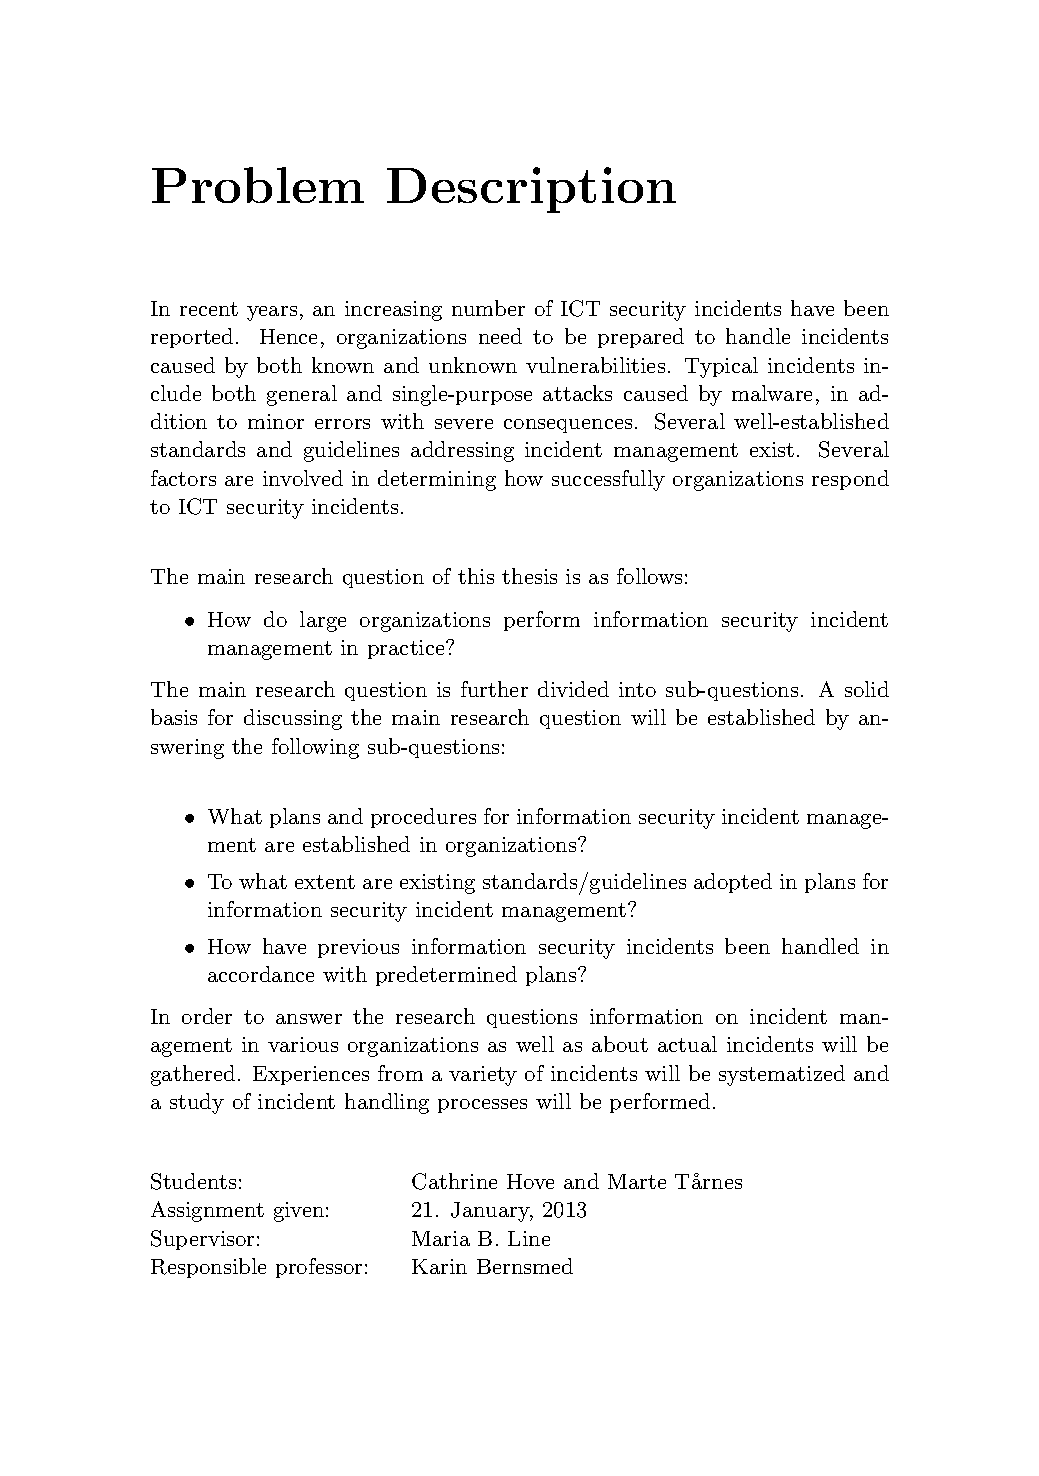
\includepdf[pages={-}]{problem-description.pdf}
\cleardoublepage
\pagenumbering{roman}
\chapter*{Abstract}
Despite the implementation of security, information security incidents occur. Preventive measures is therefore not sufficient and establishing an incident management capability is essential. In this thesis organizations' incident management practices are studied. An empirical study was conducted, including qualitative interviews and document studies of three large Norwegian organizations. The findings show that they to a large extent comply with standards and guidelines, but that there is still room for improvements. 
\cleardoublepage
\chapter*{Preface}
This master's thesis is submitted to the Norwegian University of Science and Technology (NTNU) as the last part of the five-year program Master of Science in Communication Technology at the Department of Telematics (ITEM).

We would like to thank our supervisor Maria B. Line and our professor Karin Bernsmed for valuable comments and guidance throughout this work. We would also like to thank all participating organizations and all the interviewees who took the time to participate in the case study.

Trondheim, June 6th, 2013

Cathrine Hove and Marte T\aa rnes
\cleardoublepage
\tableofcontents
\cleardoublepage
\listoffigures 
\cleardoublepage
\listoftables
\cleardoublepage
\chapter*{Acronyms}

\begin{acronym}
\acro{CIRT}{Computer Incident Response Team}
\acro{ISIRT}{Information Security Incident Response Team}
\end{acronym}
\cleardoublepage
\pagenumbering{arabic}
%Commands to create page numbering and sections/chapters on top of page
\pagestyle{fancy}
\fancyhead[LE]{\thepage \\}
\fancyhead[RE]{\leftmark \\}
\fancyhead[RO]{\thepage \\}
\fancyhead[LO]{\rightmark \\}
%Empty the footer
\fancyfoot{}

\chapter{Introduction}
In the last couple of years there has been an increased focus on incident management. Some major incidents received attention in media and have drawn attention to the topic. A few surveys exist and new standards such as ISO/IEC 27035 have emerged and several guidelines have been developed.

\section{Scope}
This thesis focus mainly on large, Norwegian organizations and how they do security incident management.\\

-large organizations, not SME.\\
-look at ICT security incidents, does not apply to other security breaches\\
-mainly focsues on norwegian organizations, kan ikke nødvendigvis si noe om resten av verden.

\section{Motivation}
Organizations are increasingly using and depending on information technology in business operations. As value and sensitivity of information increases, so does potential threats. Attacks get more advanced and attackers choose their targets more wisely. A significant challenge arise when new and severe security threats evolve faster than corresponding measures. This leads to an increasing gap between threats and security measures in organizations. To avoid severe consequences in business operations and leakage of sensitive information this gap must be closed.

A recent report\footnote{``Mørketallsundersøkelsen 2012 (Norwegian)", a survey identifying cybercrime and ICT incidents in Norwegian organizations.} published by NSR\footnote{``Næringslivets sikkerhetsråd (NSR) (Norwegian)" is a Norwegian organization with objective to prevent crime in and against business by presenting security threats and trends.} shows an increase in information espionage and cybercrime among Norwegian organizations in the last couple of years\cite{Morketall2012}. Especially targeted attacks, known as advanced persistent threats, appears to be increasing. These attacks involve industrial, political and military espionage performed by attackers with extensive resources aimed at a single organization. Typical attacks include customized e-mails containing malicious attachments or links. Hence, it is important that exposed organizations are prepared to handle such attacks and potential incidents caused by them. 

On the basis of this increasing problem, it is interesting to look at how organizations do incident management in practice. How organizations prepare for and handle incidents, comply with standards and learn from mistakes made both internally and by others are of interest. We want to assess how various factors contribute to the efficiency and effectiveness of organizations’ incident response. By identifying how these factors affect successful incident management, we hope to find improvements to incident management practice for relevant organizations. 

%Awareness among employees is important to avoid severe incidents breaking out. The \ac{NSM} made an assessment where results show that there is an overall low understanding of risks in organizations and that important measures such as risk assessment, improving skills of personnel, incident reporting and security audits are not satisfactory\cite{Morketall2012}. Through our research, we hope to draw attention to some of these challenges faced by organizations and increase awareness. 

%In recent years, trends show increase in severe ICT security incidents, more targeted and professional attacks and malware spread to and from mobile units. (Maria snakket om at SINTEF, i.e utsatt forskningsinstitusjon, hadde planer som gikk veldig langsomt å gjennomføre, kanskje vi kan gjøre noe bra her, komme med forbedringsforslag i og med at noen av våre participants i studien er i en utsatt gruppe?).

%We want to study how organizations perform information security incident management in practice because we want to assess how various factors contribute to the efficiency and effectiveness of organizations’ incident response processes. By identifying how various factors affect successful incident response, we hope to find improvements to incident management practice for organizations in the ICT sector so they might better protect against severe security incidents in the future. 

\section{Objectives}
We wish to draw attention to and increase awareness around incident management. By investigating how various organizations do incident management, what plans and procedures exist and to what extent they comply with standards, we also hope to find potential improvements.


\section{Limitations}

- few organizations, thus no statistical generalization\\
- ICT incidents, not other.\\
- norwegian?

\section{Outline}
\cleardoublepage
%To prevent footnote from splitting over two pages
%\interfootnotelinepenalty=10000
\chapter{Background}
\label{chp:background}
This chapter presents relevant background information with regards to incident management. An overview of incident management, relevant standards and guidelines as well as related research is presented.

\section{Incident Management Overview}
This section provides an overview of common concepts and terms used in incident management.
\subsection{Definitions}
\label{sec:Definitions}
%Eller et annet navn, poenget er å includere definisjoner av disse tidlig i rapporten
In information security incident management there are a few terms that need to be defined clearly. Two such terms are information or computer security \textit{incidents}\footnote{In this report the terms ``information security incident", ``computer security incident", ``ICT security incident", ``security incident" and ``incident" are used interchangeably.} and information or computer security \textit{events}. It is important to recognize these as two terms of different meaning. The standard \acs{ISO}/\acs{IEC} 27000\footnote{\acs{ISO}/\acs{IEC} 27000 Information technology -- Security techniques -- Information security management systems -- Overview and vocabulary} \cite{ISO/IEC27000} specifies the following definitions:

\textbf{Information security:} Preservation of confidentiality, integrity and availability of information; in addition, other properties such as authenticity, accountability, non-repudiation and reliability can also be involved.

\textbf{Information security event:} Identified occurrence of a system, service or network state indicating a possible breach of information security policy or failure of safeguards, or a previously unknown situation that may be security relevant.

\textbf{Information security incident:} Single or a series of unwanted or unexpected \emph{information security events} that have a significant probability of compromising business operations and threatening information security.

\textbf{\ac{ISIRT}:} Team of appropriately skilled and trusted members of the organization that handles information security incidents during their lifecycle.

The guidelines \acs{NIST} Special Publication (SP) 800-61: Computer Security Incident Handling
Guide \cite{nist800-61} specifies the following definitions:

\textbf{Event:} An event is an observable occurrence in a system or network.

\textbf{Adverse event:} Adverse events are events with a negative consequence, such as system crashes, packet floods, unauthorized use of system privileges, unauthorized access to sensitive data, and execution of malware that destroys data.

\textbf{Computer security incident:} A violation or imminent threat of violation\footnote{An ``imminent threat of violation" refers to a situation in which the organization has a factual basis for believing that a specific incident is about to occur.} of computer security policies, acceptable use policies, or standard security practices.

\acs{NorCERT} specifies the following definitions \cite{NorCERT3Kvartal2012}:

\textbf{\ac{CSIRT}:} A central tool with the task of protecting important infrastructure. The team must consist of security specialists and they must handle and responds to incidents. Additionally, they need to create awareness and educators.

\textbf{\ac{CERT}:} A trademark that can only be used after approval by Carnegie Mellon University. Is in practice the same as a \acs{CSIRT}.

The definition of an adverse event from \acs{NIST} \cite{nist800-61} is quite similar to the definition of information security event from ISO/IEC \cite{ISO/IEC27000}. The definitions of incidents are also quite similar. These definitions are the ones that will be used in this report. \ac{ISIRT}, \ac{CSIRT} and \ac{CERT} define similar types of teams. In this report the term \acs{IRT} is used to denote such a team. 

\subsection{What is Incident Management}
Incident management is a collective term composing all activities associated with managing security incidents. Incident management is not restricted to incident handling alone, but includes activities for the entire incident lifecycle; from planning, training and raising awareness to detecting, responding and learning from incidents. 

Various guidelines and standards describe best practice and suggest activities for effective and efficient incident management. It is important to note that incident response requires a substantial amount of planning and resources. Two of the most important parts of incident management are the existence of guidelines for communication and prioritization of incidents as well as the use of a evaluation process to gain experience from previous incidents. \cite{nist800-61}

As part of an incident management capability, organizations should have an incident management policy, a plan and procedures, all of which should be tailored to the specific organization's needs. Additionally, it is important to have a planned approach to reporting of vulnerabilities that have not yet been exploited. \cite{ISO/IEC27035}

%The policy should include definitions, forms and commitment from senior management, plans should outline the organization's approach towards incident response, whereas procedures should be based on the current incident management policy and plan.

%\acp{SOP} are a delineation of the specific technical processes, techniques, checklists and forms used by the incident response team. An organization should establish procedures regarding communication with various outside parties, like media, law enforcement, other incident response teams, software vendors and \acp{ISP}. It is common to have \acp{PoC} for the various outside parties. \cite{nist800-61}

Incident management is not purely an IT related issue as information security incidents threaten an organization as a whole. Having a well-planned and tailored incident management capability is therefore important for organizations in order to protect information. Incident management seeks to both prevent, contain and resolve incidents, in addition to post-learning. ENISA states the following about incident management \cite{enisaGuide}: 

\begin{quote}
\textit{``Incident management is an important tool of overall governance and to have it, in whatever form or shape, is a necessity."}
\end{quote}

\subsection{\acl{IRT}}
Having an \ac{IRT} will aid organizations in responding to incidents more effectively and efficiently, in addition to providing a structured approach for learning from previous incidents. 

As the various definitions in section \ref{sec:Definitions} indicate, an incident response team is ``a team that responds to computer security incidents by providing all necessary services to solve the problem(s) or to support the resolution of them" \cite{enisaCSIRTGoodPractices}. The team structure, members, tasks and responsibilities may vary depending on organizations' resources and needs. 

\ac{NIST} recommends having one person in charge of incident response, taking the role as team manager. The team manager should act as a liaison to senior management as well as ensuring that the team has the necessary resources, personnel and skills. It is recommended that team members have diverse backgrounds so they can handle different incidents that occur. The team manager should assess the situation and assign responsibility for incidents to the most appropriate team member. \cite{nist800-61}

Usually teams consist of highly technically skilled persons, and teams should have at least one member with expertise in each major technological category. Good problem solving skills and communication skills are essential to the team as effective incident response require collaboration and coordination within the team and throughout the organization. \cite{nist800-61}

The structure of the team may vary. The number and frequency of incidents as well as team responsibilities should guide organizations' choice of team structure. However, whenever justified  the ISO/IEC 27035 standard\footnote{ISO/IEC 27035 Information technology - Security techniques - Information security incident management} recommends having a permanent team. \cite{ISO/IEC27035}

%\acp{IRT} should have clearly defined responsibilities, processes, allocation of roles and appropriate training programs\cite{ISO/IEC27035}. Team members should hold appropriate access permissions and have access to supportive tools to be best prepared to perform incident response \cite{SANShandbook}.
%

Participating in a community of teams will be beneficial for teams due to collaboration on standards and procedures as well as information and resource sharing. To minimize the frequency of incidents and to mitigate negative impact caused by them, most \acp{IRT} do not only provide reactive services, but may also have other responsibilities, such as intrusion detection, advisory distribution, education and raising awareness within the organization. \cite{nist800-61}  
  
\section{Standards and Guidelines}
This section gives an introduction to the most relevant and widely implemented standards and guidelines for information security incident management. 
\label{section:standardsandguidelines}
\subsection{The \acs{ISO}/\acs{IEC} 27001 Standard}
\label{sec:iso27001}
This standard provides a model for establishing, implementing, operating, reviewing, maintaining and improving an \ac{ISMS}. It states that management shall provide evidence of its commitment to the ISMS. This section presents clauses relevant to incident management that are directly retrieved from the standard \cite{ISO/IEC27001}. 

\textbf{4.2.2 Implement and operate the \ac{ISMS}} \\
The organization should do the following.
\begin{enumerate}[h)]
\item Implement procedures and other controls capable of enabling prompt detection of security events and response to security incidents.
\end{enumerate}

This clause specifies that organizations should be able to detect and handle security incidents.

\textbf{4.2.3 Monitor and review the ISMS}\\
The organization shall do the following.
\begin{enumerate}[a)]
\item Execute monitoring and reviewing procedures and other controls to:
\begin{enumerate}[2)]
\item promptly identify attempted and successful security breaches and incidents;
\end{enumerate}
\vspace{-0.2cm}
\begin{enumerate}[4)]
\item help detect security events and thereby prevent security incidents by the use of indicators;
\end{enumerate}
\vspace{-0.2cm}
\begin{enumerate}[5)]
\item determine whether the actions taken to resolve a breach of security were effective.
\end{enumerate}
\item Undertake regular reviews of the effectiveness of the \ac{ISMS} (including meeting \ac{ISMS} policy and objectives, and review of security controls) taking into account results of security audits, incidents, results from effectiveness measurements, suggestions and feedback from all interested parties.
\end{enumerate}

\textbf{4.3.3 Control of records}\\
Records shall be kept of the performance of the process as outlined in 4.2 and of all occurrences of significant security incidents related to the \ac{ISMS}

Common for all clauses in this standard is that they only specify that things should be done, and not \textit{how} they should be done. The \acs{ISO}/\acs{IEC} 27002 standard\footnote{ \acs{ISO}/\acs{IEC} 27002 Information technology - Security techniques
- Code of practice for information security management} provides a code of practice for information security management and the \acs{ISO}/\acs{IEC} 27035 standard provides guidelines for the establishment of information security incident management. These standards are further described in sections \ref{sec:iso27002} and \ref{sec:iso27035} and can be used as aids to fulfil the clauses presented in the \acs{ISO}/\acs{IEC} 27001 standard.
\subsection{The \acs{ISO}/\acs{IEC} 27002 Standard}
\label{sec:iso27002}
This standard represents a code of practice for information security management and establishes guidelines for initiating, implementing, maintaining and improving information security management in an organization. The standard is intended to be a starting point for developing organization specific guidelines and contains 11 security control clauses that outline various security objectives and provide implementation guidance. It is emphasized that organizations should initially identify and establish their security requirements and then choose which of the security controls to implement.

This section presents clauses from the standard that are relevant to incident management. They are retrieved from \cite{ISO/IEC27002}.

\textbf{13.1 Reporting information security events and weaknesses } \\
The objective is to ensure that all significant information security events and weaknesses are reported such that corrective actions can be made in time. Reporting procedures and employee awareness are important success factors and it should be required to report any events or weaknesses to the point of contact as quickly as possible.

\textbf{13.1.1 Reporting information security events} \\
\emph{Control:} Information security events should be reported through appropriate management channels as quickly as possible.

\emph{Implementation guidance:} A point of contact and a formal event reporting procedure should be established and employees should be made aware of these. The reporting procedure should include the following.
\begin{enumerate}[a)]
\item suitable feedback processes to ensure that those reporting information security events are notified of results after the issue has been dealt with and closed.
\item information security event reporting forms to support the reporting action, and to help the person reporting to remember all necessary actions in case of an information security event.
\item the correct behaviour to be undertaken in case of an information security event.
\item reference to an established formal disciplinary process for dealing with employees, contractors or third party users who commit security breaches.
\end{enumerate}

\textbf{13.1.2 Reporting security weaknesses} \\
\emph{Control:} All employees, contractors and third party users of information systems and services should be required to note and report any observed or suspected security weaknesses in systems or services.

\emph{Implementation guidance:} There should exist an easy, accessible and available reporting mechanism for employees, contractors and third party users. Weaknesses should be reported as quickly as possible to either management or the service provider and not attempted to be proven.

\textbf{13.2 Management of information security incidents and improvements}\\
The objective is to ensure that the management of security incidents follows a consistent and effective approach where responsibilities and procedures are in place to handle incidents once they have been reported. Procedures should be in place for continual improvement of management processes. When necessary to collect evidence, this should be done in compliance with legal requirements.

\textbf{13.2.1 Responsibilities and procedures}\\ 
\emph{Control:} Management responsibilities and procedures should be established to ensure a quick, effective and orderly response to information security incidents.

\emph{Implementation guidance:} In addition to reporting, monitoring should be used to discover incidents. When implementing incident management procedures organizations should consider the following.
\begin{enumerate}[a)]
\item procedures should be established to handle different types of information security incidents, including:
\begin{enumerate}[1)]
\item information system failures and loss of service.
\item malicious code.
\item denial of service.
\item errors resulting from incomplete or inaccurate business data.
\item breaches of confidentiality and integrity.
\item misuse of information systems.
\end{enumerate}
\item in addition to normal contingency plans, the procedures should also cover:
\begin{enumerate}[1)]
\item analysis and identification of the cause of the incident.
\item containment.
\item planning and implementation of corrective action to prevent recurrence, if necessary.
\item communication with those affected by or involved with recovery from the incident.
\item reporting the action to the appropriate authority.
\end{enumerate}
\item audit trails and similar evidence should be collected and secured, as appropriate, for:
\begin{enumerate}[1)]
\item internal problem analysis.
\item use as forensic evidence in relation to potential breach of contract or regulatory requirement or in the event of civil or criminal proceedings, e.g. under computer misuse or data protection legislation.
\item negotiating for compensation from software and service suppliers.
\end{enumerate}
\item action to recover from security breaches and correct system failures should be carefully controlled. The procedures should ensure that:
\begin{enumerate}[1)]
\item only certain identified and authorized personnel are allowed access to live systems and data.
\item all emergency actions taken are documented in detail.
\item emergency action is reported to management and reviewed in an orderly manner.
\item the integrity of business systems and controls is confirmed with minimal delay.
\end{enumerate}
\end{enumerate}

\textbf{13.2.2 Learning from information security incidents}\\
\emph{Control:} There should be mechanisms in place to enable the types, volumes, and costs of information security incidents to be quantified and monitored.

\emph{Implementation guidance:} By monitoring incidents, reoccurring and high impact incidents can be identified and need for additional controls can be evaluated.

\textbf{13.2.3 Collection of evidence}\\
\emph{Control:} Where a follow-up action against a person or organization after an information security incident involves legal action (either civil or criminal), evidence should be collected, retained, and presented to conform to the rules for evidence laid down in the relevant jurisdiction(s).

\emph{Implementation guidance:} The rules of evidence involve admissibility and weight of evidence, that is whether or not evidence can be used in court and the quality and completeness of the evidence. To achieve admissibility and weight of evidence, organizations should ensure their systems comply with standards and that controls used to protect evidence are complete and consistent.

\subsection{\acs{ISO}/\acs{IEC} 27035}
This section gives an introduction to the ISO 27035 standard and the content is, unless specified otherwise, derived from \cite{ISO/IEC27035}. 

Implementing this standard will aid organizations in dealing with information security incidents properly and mitigate both direct and indirect adverse business impact. This standard provides an extensive and structured approach towards incident management by presenting five phases with recommended activities for large and medium-sized organizations. 

One of the standard's objectives is to provide guidelines to aid organizations in meeting the requirements specified in ISO/IEC 27001. %For this purpose a cross-reference table showing how following the guidelines in ISO/IEC 27035 fulfils the requirements in ISO/IEC 27001 is given in the appendix.

\paragraph{Plan and Prepare} This phase is by far the most extensive phase and involves many activities. Individual organizations have to ensure that their use of resources are proportional and according to their needs. Each organization should formulate an incident management policy reviewing current vulnerabilities, stating the need for an incident management scheme and identifying overall benefits for the organization. Security and risk management policies should be reviewed and updated regularly. The standard highlights the importance of ensuring commitment from senior management in the security incident management policy to ensure the organization's commitment to resources and maintenance of an incident management capability.  

One main activity in the plan and prepare phase is making a detailed incident management scheme that contains forms, procedures and support tools for the detection and reporting of, assessment and decision making related to, making responses to and learning lessons from incidents. The scheme should include a classification scale for grading incidents and reporting forms (preferably electronic).   

An important activity in this phase is the establishment of the \acf{ISIRT}. Organizations should also establish and implement required mechanisms of support for their incident management scheme to operate efficiently during this phase. This includes technical tools such as IDS and log monitoring systems as well as relationships and connections to other organizations. 

It is essential for the success of a structured incident management approach that awareness and participation of all personell is present. All personell should be familiar with the incident management scheme when it comes operational and be able to recognize its benefits. It is therefore recommended that an appropriate awareness and training program is developed and repeated from time to time as personell change over time.

The entire incident management scheme should be tested to verify that the scheme and \ac{ISIRT} work in complex and real situations. When this phase is completed, organizations should be fully prepared to manage security events, incidents and vulnerabilities that occur.

\paragraph{Detection and Reporting} The first operational phase of an incident management scheme involves detection, collection of information and reporting of occurrences of security events, incidents and vulnerabilities either discovered by humans or automated systems. It is important to preserve information about vulnerabilities and incidents in a database operated and maintained by the \ac{ISIRT}. Organizations should implement security monitoring systems, \acl{IDS}/\acl{IDP} (\acs{IDS}/\acs{IDP}), antivirus programs and so forth to aid the detection of security events, incidents and vulnerabilities. Logs from various entities should be analysed and registrations of incidents should be made in an Incident Tracking System. 

It is the person first notified about an event that is responsible for starting the activities involved in this phase. There are several ways a security event or incident can be discovered and thus all personell should be aware of and have access to the guidelines for reporting. There should be clear procedures to follow for the people involved in dealing with an incident. All relevant information should be passed to the PoC and the responsible \ac{ISIRT} member. It is recommended that one of the \ac{ISIRT} members are appointed the responsibility for incoming reports and makes an assessment for further actions.  A reporting form should be specified to ensure that all necessary and relevant information is preserved and that there is consistency in information gathered. 

\paragraph{Assessment and Decision} This phase includes assessment of information regarding security events and decisions on whether events should be treated as incidents. The assessment and decision phase also includes assessment of information received regarding vulnerabilities and decisions of how to handle these in accordance with previously agreed actions.

The PoC should use a predefined classification scale to make an assessment of security events, whether they are incidents or false alarms and what impact they may have on the organization's core services, information and affected assets. The initial assessment made by the PoC should be verified by an \ac{ISIRT} member. \ac{ISIRT} makes decisions about how the incident should be handled, by whom and in what priority. To be able to respond to security incidents in an efficient and effective way, a prioritizing process should be conducted based on the level of adverse business impact and the required effort to solve them.  All information pertaining to an incident should be recorded in the database by \ac{ISIRT}. A main activity for the \ac{ISIRT} is to allocate responsibilities for incident management actions and provide thorough and structured procedures for persons involved to follow. 

\paragraph{Responses} The third operational phase presents guidelines and activities for organizations in responding to security incidents. The response should be in accordance with the actions agreed in the previous phase, whether it is an immediate, real-time or near real-time response or involves forensics analysis. This phase also involves making responses to vulnerabilities reported either internally or by other parties. As a first step the \ac{ISIRT} has to determine whether the incident is under control, and then initiate the appropriate actions. For situations out of control, escalation to crisis handling might be necessary for further assistance. Otherwise, the response work such as recovery, proper documentation and communication to relevant parties can be started. 

The \ac{ISIRT} should consider which internal and possibly external resources to utilize for best responding to incidents. It is important that every action conducted by the \ac{ISIRT} in this phase is logged properly and that guidelines are used to ensure thorough documentation. Logging actions will aid in analysing how effective and efficient the incident response process was as well as ensuring that any possible evidence is not compromised. It is the \ac{ISIRT}'s responsibility to make sure the affected assets become operational again and that they are not vulnerable to the same attack. Once an incident has been handled successfully, the case should be closed formally by the \ac{ISIRT} and recorded in the database.

\paragraph{Lessons Learned} The final phase starts after an incident has been resolved and/or closed and focuses on analysing whether the organization's incident management scheme worked successfully. During this phase improvements are identified and made. One of the main activities is reviewing how effective the entire incident management process was in responding to, assessing and recovering from the incident. Shortcomings and improvements in policies, procedures, security control implementations, reporting formats and risk assessments should be identified during this phase. Improvements may be implemented immediately or incorporated into future plans. The \ac{ISIRT} should make sure improvements are made to the entire system and not only the affected parts.

The lessons learned phase has many iterative activities. An essential post-incident activity is documenting incidents properly, ensuring incident trend analysis is accurate. Sharing experiences with trusted communities and partners should be done on a regular basis, regardless of whether incidents occur internally. Reviews, trend analysis and testing should be performed frequently to ensure regularly improvements to the incident response scheme over time. 





\subsection{ITIL}
\label{section:ITIL}
\ac{ITIL} is a framework and a source of good practice for service management, which is aligned with \acs{ISO}/\acs{IEC} 27000. This section gives a brief introduction to \ac{ITIL}, focusing on the parts related to incident management and the content is, unless specified otherwise, derived from \cite{itilbok}. The definitions presented in this section are taken directly from \cite{itilbok}.

To describe service management, the \ac{ITIL} framework uses the following definitions:

\textbf{Service:} A service is a means of delivering value to customers by facilitating outcomes that customers want to achieve without the ownership of specific costs and risks.

\textbf{Service Management:} Service management is a set of specialized organizational capabilities for providing value to customers in the form of services.

The specialized organizational capabilities include the processes, activities, functions and roles that a service provider uses in delivering services. The \ac{ITIL} framework is generic and is meant to be useful for any type of organization. It describes a set of functions and processes that can be implemented in order to be able to perform service management. The terms function and process are defined in the following ways:

\textbf{Function:} A team or group of people and the tools they use to carry out one or more processes or activities.

\textbf{Process:} A process is a structured set of activities designed to accomplish a specific objective. A process takes one or more defined inputs and turns them into defined outputs. A process may include any of the roles, responsibilities, tools and management controls required to reliably deliver the outputs. A process may define policies, standards, guidelines, activities and work instructions if they are needed.

%Risk is defined as a possible event that could cause harm or loss, or affect the ability to achieve objectives. Risk can also be defined as the uncertainty of outcome.

This section describes processes and functions related to incident management.

\paragraph{Availability Management}
Availability management is essential for an organization and is primarily a proactive process. In addition to activities such as preparing and maintaining an availability plan and monitoring availability levels, this process includes assisting investigation and resolution of availability related incidents and problems. The latter is a reactive part of availability management. This process is related to other processes including IT service continuity, information security, event, incident and problem management.

\paragraph{IT Service Continuity Management}
This process is concerned with key systems in the event of a failure. The purpose of the process is to ensure that IT resources, systems and services can be restored within agreed timescales in the event of a major incident. The process is related to availability and information security management.

\paragraph{Information Security Management}
This process is concerned with enforcing the security policy. The system in place for this is the \ac{ISMS}. The security policy in an organization is something everyone should have access to and be aware of. Information security management is related to availability, incident, problem and IT service continuity management. 

\paragraph{The Service Desk}
The service desk is a function. One of the processes the service desk carries out is incident management. The service desk should be the single point of contact for IT users in an organization. This means that if users wish to log incidents or report events they should contact the service desk. The service desk is the owner of incidents throughout their lifecycle, regardless of who is working on the incident. They should be trained to obtain the skills needed in order to perform incident management as effectively and efficiently as possible.

\paragraph{Incident Management}
This is the process for dealing with incidents. An incident is defined as being an unplanned interruption to an IT service or reduction in quality of an IT service. An incident can also be the failure of a configuration item that has not yet impacted service. Hence, incident management includes both incidents where service has been disrupted or where service has not yet been disrupted. Each organization should have its own definition of a major incident. Large organizations may have dedicated teams available 24/7 to handle major incidents. 

\begin{sidewaysfigure}
\centering
\scalebox{0.45}
{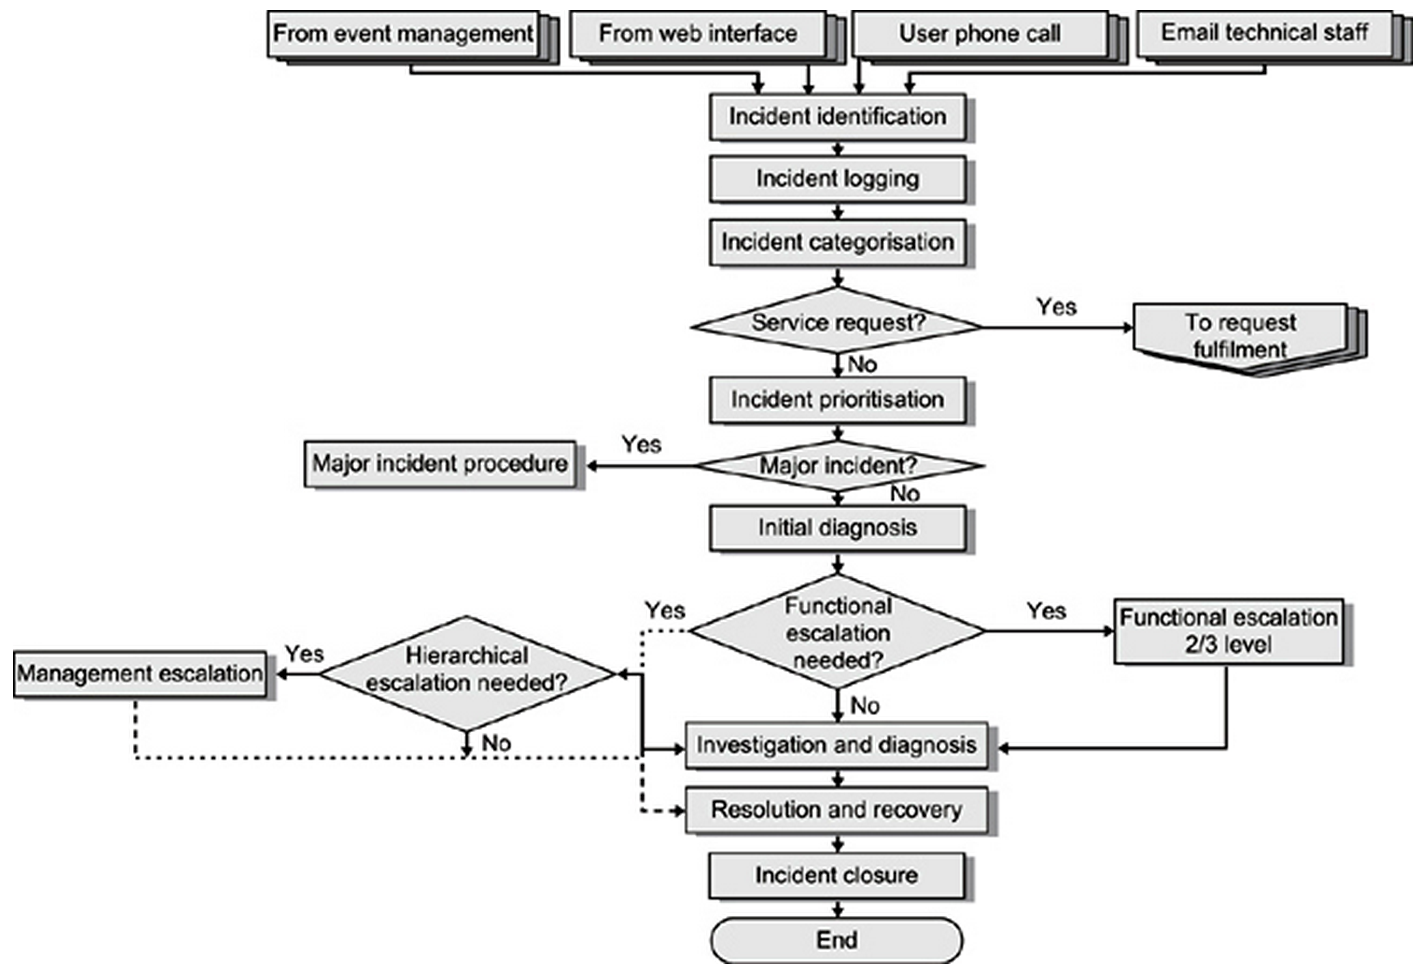
\includegraphics{ITILIncidentManagement.png}}
\caption[The ITIL Incident Management Process]{Incident Management Process \cite{itilbok}} 
\label{fig:ITILIncidentManagement}
\end{sidewaysfigure}

\pagebreak
In the incident management process resources are allocated to minimize and mitigate the impact of incidents and service unavailability in line with business priorities. The main objectives are to restore service as quickly as possible in addition to limit adverse impact on business operations. Incident handling may reveal areas that are in need of improvement. Organizations can adopt incident models, which are methods for handling groups of similar incidents.

The incident management process flow is illustrated in figure \ref{fig:ITILIncidentManagement}. The figure shows that incident reports can come from various sources. The incident reported needs to be identified, logged, categorized and prioritized. Accurate categorization is important as areas of the infrastructure where incidents occur can be highlighted. An example of an incident priority coding system can be seen in figure \ref{fig:ITILIncidentPrioritization}.

\begin{figure}[ht]
\begin{center}
\hspace{-0.2cm}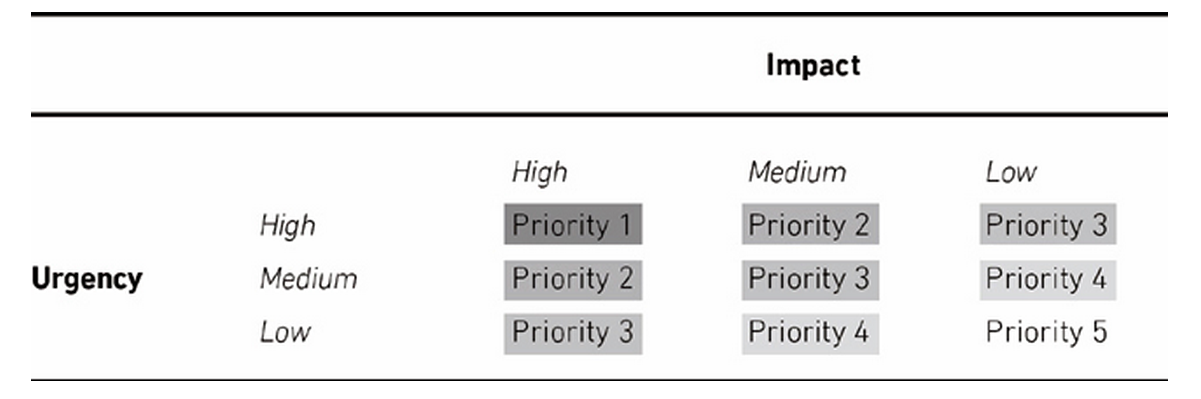
\includegraphics[scale=0.4]{ITILIncidentPrioritization.png}
\caption[ITIL Incident Priority Coding System]{Incident Priority Coding System \cite{itilbok}}
\label{fig:ITILIncidentPrioritization}
\end{center}
\end{figure}

If the incident turns out to be major, the major incident process is initiated. The incident handling may also need to be escalated. Functional escalation is when the service desk is not able to resolve the incident or when they have not been able to resolve it within the target resolution time. Hierarchical escalation is when the profile of a specific incident within the IT organization and also within business areas needs to be raised. Any incident needs to be investigated and diagnosed in order to subsequently be resolved and closed. The incident management process is closely related to the problem management process.

\begin{figure}[H]
\hspace{-1cm}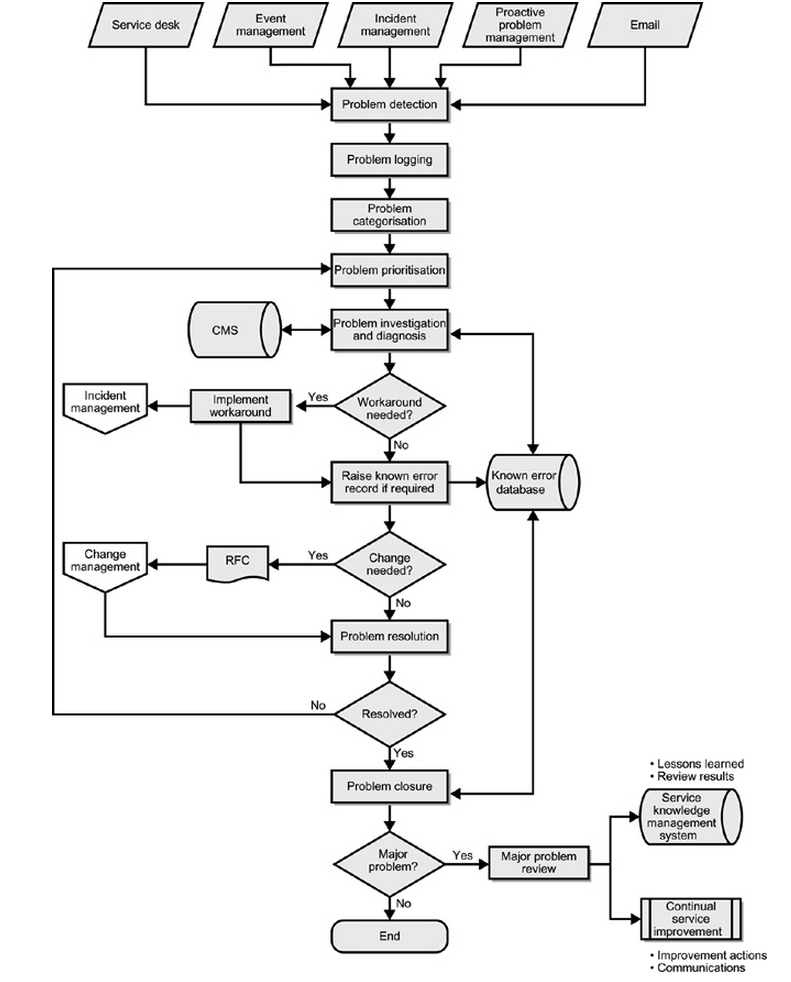
\includegraphics[scale=0.68]{ITILProblemManagement.png}
\caption[The ITIL Problem Management Process]{Problem Management Process \cite{itilbok}}
\label{fig:ITILProblemManagement}
\end{figure}

\paragraph{Problem Management}
The problem management process concerns analysis of the root cause as well as the resolving of problems. A problem is defined as being the cause of one or more incidents. The process is both proactive and reactive and seeks to prevent problems and incidents as well as reduce the impact of those that cannot be prevented. The problem management process is illustrated in figure \ref{fig:ITILProblemManagement}. 

The figure shows the various inputs to the process. It is important to log all details of the problem. Each problem needs to be categorized and prioritized. They should be prioritized in the same way as incidents, e.g. as in figure \ref{fig:ITILIncidentPrioritization}. During investigation and diagnosis the root cause of the problem should be discovered. The problem needs to be resolved as soon as a permanent fix is available and subsequently closed. If the problem is major, a major problem review must be conducted.

\paragraph{Event Management}
The event management process handles normal messages and detects, escalates and reacts to exceptions. An event can be informational, a warning or an exception. The event management process is similar to the incident management process and should ideally be automated. Some events are triggers for the incident management process.
%CI - Configuration Item
\subsection{\acs{NIST} Special Publication 800-61}
This subsection gives an introduction to the guidelines \acs{NIST} SP 800-61 and the content is, unless specified otherwise, derived from \cite{nist800-61}. This publication aims to  assist organizations in mitigating risks from computer security incidents by providing guidelines on how to respond to incidents effectively and efficiently. 

One of the first considerations for a \ac{CSIRC} should be to agree on a definition of the term incident. This guidelines' definitions of events and incidents are included in section \ref{sec:Definitions} of this report. 

\acs{NIST} SP 800-61 describes the four phases of incident response; preparation, detection and analysis, containment, eradication and recovery and post-incident activity. The phases and the relationship between them are illustrated in figure \ref{fig:NISTIncidentResponse}.

\begin{figure}[ht]
%\hspace*{-0.4cm}
\begin{center}
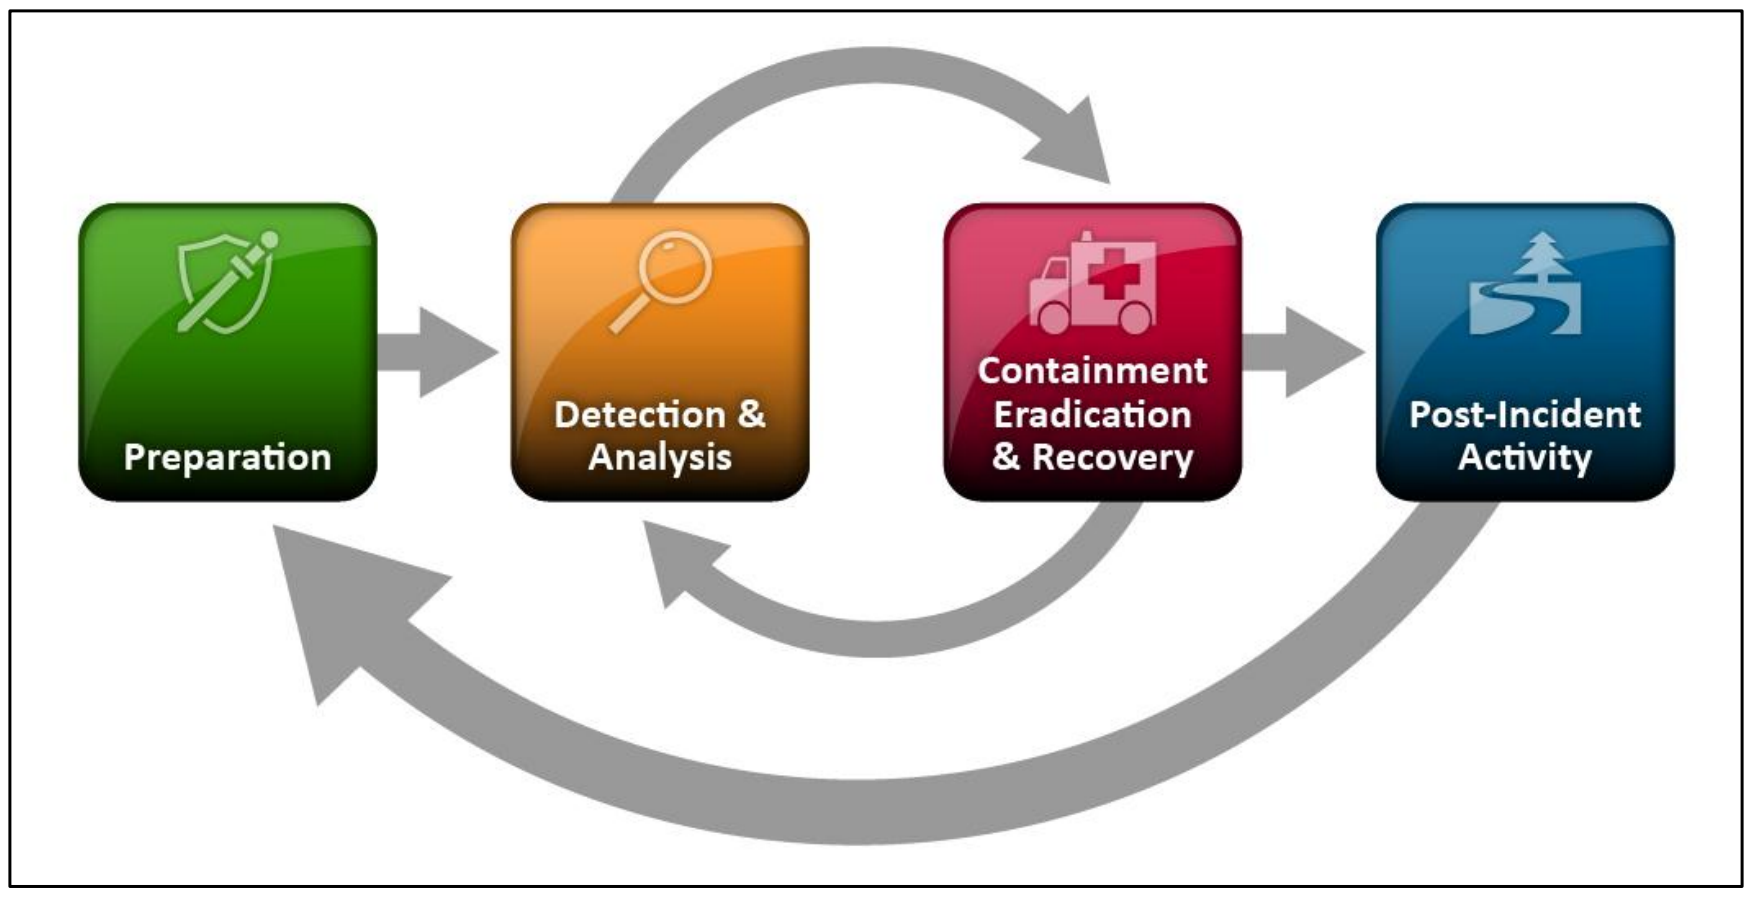
\includegraphics[scale=0.27]{NISTIncidentResponseCycle.png}
\caption[The Incident Response Life Cycle]{The Incident Response Life Cycle \cite{nist800-61}}
\label{fig:NISTIncidentResponse}
\end{center}
\end{figure}

\paragraph{Preparation} 
This phase includes establishing an incident response capability as well as preventing incidents. The latter is not typically a part of the incident response team's tasks, but it is fundamental to the success of the organization's incident response. If a large number of incidents occur, it may overwhelm the incident response team. To prepare for incidents the incident handlers should have tools and resources like contact information, incident reporting mechanisms, issue tracking system, digital forensic workstations\footnote{A digital forensic workstation is specially designed for acquiring and analysing data. It usually contains a set of removable hard drives that can be used for evidence storage.} and digital forensic software. It is common to create a portable \emph{jump kit} containing materials that may be needed during incident response.

\paragraph{Detection and Analysis}
Organizations should prepare to handle any type of incident and to handle common incident types. A classification of incidents can be used as a basis for incident handling. The guidelines provides a list of example categories for incidents that contains web, email, improper usage and loss or theft of equipment. This guidelines focuses on handling of any type of incident and not specific categories. A challenge related to incident handling is to detect the incident and determine the potential impact the incident may have. The actual detection may be the hardest part of incident handling. The guidelines defines two types of signs of incidents; precursors and indicators, with indicators being the most common. These are defined in the following way: "A \emph{precursor} is a sign that an incident may occur in the future. An \emph{indicator} is a sign that an incident may have occurred or may be occurring now." Common sources for precursors and indicators are \acp{IDPS}, antivirus and antispam software, third-party monitoring services, logs, information on new vulnerabilities and exploits and people. 

A challenging part of this phase is the analysis, i.e. to determine which indicators and precursors are legitimate, if they are really related to an incident and what has actually happened. When the team believes an incident to have occurred they should try to determine the scope. All steps taken should be documented and timestamped. It is important to note that any such documentation can be used in court. The incident response team should maintain a database containing information about incidents, such as status, indicators, related incidents and actions taken by the incident handlers. It is important to prioritize incidents and handle them accordingly. Factors that can be used as a basis for prioritization include the functional impact of the incident, the information impact of the incident and recovery from the incident. When the prioritization is performed the incident response team should notify the appropriate people. It is important to have procedures regarding who these people should be.

\paragraph{Containment, Eradication and Recovery}
Containment is obviously an important part of incident handling. The existence of strategies and procedures for containment is helpful. These strategies and procedures are different for different types of incidents. Gathering and handling of evidence is part of this phase. For some incidents eradication is necessary and for some it is done during recovery. Eradication can include deleting malware and disabling breached user accounts. Recovery consists of restoring systems to normal operation and in some cases eliminate vulnerabilities that could have causes similar incidents. The guidelines does not offer specific recommendations for eradication and recovery as these are often OS specific. 

\paragraph{Post-Incident Activity}
Learning and improving is one of the most important parts of incident response. It is recommended to hold a ``lessons learned" meeting after each major incident and periodically after lesser incidents. One meeting could cover several incidents. ``Lessons learned" meetings should generally focus on revealing what was done well and what could be improved. The desired result is that the organization will be better equipped for the next incident that occurs. Often incident response policies and procedures are updated. The areas these meetings should focus on include how well the staff performed and what they could have done differently, if documented procedures were followed and if they were adequate and how information sharing with other organizations could have been improved. To prevent future similar incidents potential corrective actions and potential additional tools and resources should be reviewed. Both people involved in the incident(s) in question and people needed for future cooperation should be included in these meetings. A follow-up report that provides a reference that can be used when handling future similar incidents should be created. Other post-incident activities include the use of collected data for risk assessment, measurement processes to determine the success of the incident response team and audits of incident response programs. 




\subsection{\acs{ENISA} - Good Practice Guide for Incident Management}
This guide is developed by the \ac{ENISA} and provides a description of good practices for security incident management. The content is, unless specified otherwise, derived from \cite{enisaGuide}. The focus of this guide is IT and information security incidents. It specifically addresses the incident handling part of incident management. The incident management and incident handling processes are illustrated in figure \ref{fig:ENISAIncidentManagement}. The incident handling process has four major components, as shown in the figure. 

\begin{figure}[h]
\begin{center}
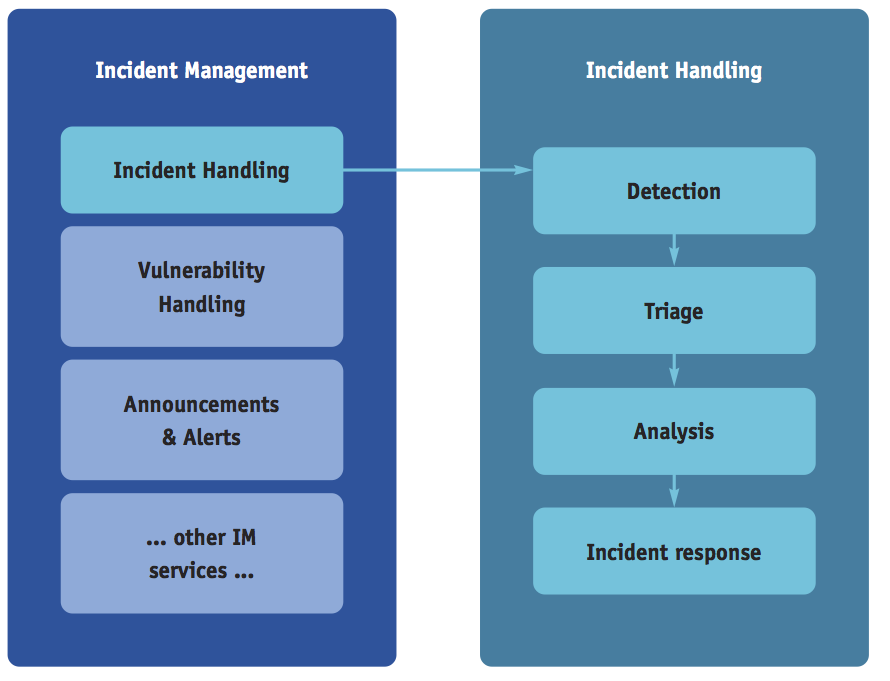
\includegraphics[scale=0.74]{enisaIncidentManagement.png}
\caption[ENISA Incident Management and Incident Handling]{Incident Management and Incident Handling \cite{enisaGuide}}
\label{fig:ENISAIncidentManagement}
\end{center}
\end{figure}

\paragraph{Detection:} The \ac{CERT} can receive incident reports from various sources. This guide recommends to use e-mail as a communication channel as people prefer this. Additionally, it recommends to use monitoring systems in addition to reports sent by others. Detection includes registration of incident reports in an incident handling system. This stage is a good place to implement pre-filtering mechanism for incident reports. The registration process could include the use of an incident report form.

\paragraph{Triage:} This stage consists of the three phases verification, initial classification and assignment. During these phases the following questions should be answered:

\begin{itemize}\itemsep-0.2cm
\item Is it really an IT security incident?
%\item Is it related to one of your constituents?
%\item Does it fit within the mandate the \ac{CERT} has?
\item What is the impact?
\item Is there collateral damage?
%\item How fast could it spread to other constituents?
\item How many people do you need to handle this incident?
\item Which incident handler should be appointed to the incident?
\end{itemize}

The verification phase seeks to answer the first question. It is however recommended to respond to and archive all reports, even those not defined as information security incidents. They may include information relevant to other incidents or potentially lead to an incident. After an incident report has been verified the incident should be initially classified according to a classification schema. The last part of the triage component is to assign the incident to an incident handler.

\paragraph{Analysis and Incident response:} These components are illustrated by figure \ref{fig:IncidentResolutionCycle}. The cycle may need to be iterated several times. To perform \textit{data analysis} there should be collected as much data as possible. Prior to the collection, all involved parties should be notified. Sources for data collection could be an incident reporter, monitoring systems, a referring database and relevant log files. The collected data should be used to try to determine the source of the incident. Prior to the data analysis, decisions about what data to analyse and in what order must be made. During the analysis, people will often exchange ideas and observations as well as draw conclusions. This belongs to the \textit{resolution research}. It is recommended to advise team members to write down any observations that can be discussed in review meetings. The \textit{action proposed} part consists of preparing a set of tasks for each party involved. The \textit{action performed} should be monitored, where possible. The main goal for all actions is the \textit{eradication and recovery}.

\begin{figure}[h]
\begin{center}
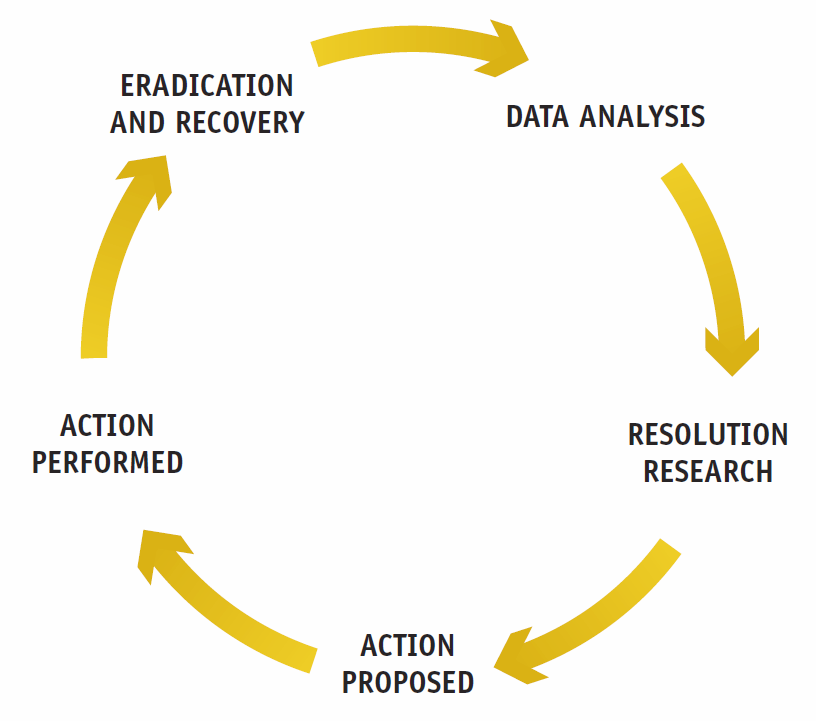
\includegraphics[scale=0.4]{IncidentResolutionCycle.png}
\caption[ENISA Incident Resolution Cycle]{Incident Resolution Cycle \cite{enisaGuide}}
\label{fig:IncidentResolutionCycle}
\end{center}
\end{figure}

When you have left the incident resolution cycle, there are still tasks to perform. The incident needs to be closed properly. Each involved party needs to be informed that the incident is resolved. The classification of the incident should be revisited and a final classification should be performed. The classification could have been revisited during the resolution cycle as well. It is recommended to have a taxonomy and to classify incidents in accordance with it.

After an incident has been resolved or closed a post-analysis should be performed in order to learn from the incident. It is also recommended not to analyse all incidents, but only the most characteristic and complex ones and those that include new attack vectors. 

Incidents should be reported to the management. In addition to specific issues, the daily operations should be reported, including costs, positive results, plans and risks. This will save time and resources in situations where you need the management's operational or financial support and quick decisions.





\subsection{NorSIS - Guideline for Incident Management}
\label{sec:NorSIS}
The \ac{NorSIS} has in cooperation with a group of students\footnote{The students did a survey on incident management in Norwegian \acsp{SME}\cite{sand2010hendelseshaandtering}} developed a guideline for incident management, published in 2010\cite{norsisveiledning}. The aim of this guideline is to give a thorough description of why and how organizations should plan for security incident management, conduct business impact analysis and explain various measures to improve information security in organizations. This guideline is specifically developed for \acp{SME} and may thus not be extensive enough for large organizations. The content in this section is, unless specified otherwise, derived from\cite{norsisveiledning}.

\paragraph{Incident Management Policy} 
An incident management policy should form the basis for developing new incident management plans in organizations. A solid policy should state an organization's objectives for incident management and include a statement ensuring commitment from senior management. Any relevant laws, standards and regulations should be included. It is essential that the policy has requirements for performing regular risk assessments, business impact analysis, tests and training. The guideline recommends to include the assignment of roles and responsibilities in the incident management policy.

\paragraph{Business Impact Analysis}
NorSIS recommends organizations to conduct a business impact analysis to identify which services are of significant value and needs to be secured. Risk assessments and the identification of possible consequences of security incidents are part of this process. The guideline emphasizes the importance of knowing risks and potential threats.  

\paragraph{Preventive Measures}
One of the most cost effective ways to perform incident management is implementing preventive measures. Listed as minimum requirements are antivirus, logs, firewalls, backups, alarms, locks, regular reviews of the threat landscape, and reporting systems for employees. Other proposed measures include encryption of data and wireless networks.   

\paragraph{Recovery Strategies}
The guideline recommends having a recovery strategy to quickly re-establish business operations after an incident. Suggestions include backup and emergency solutions. Routines and plans should be in place to handle recovery efficiently.

\paragraph{Incident Management Plan}
Organizations should use previous assessments and proposed incident scenarios to develop an incident management plan. It is recommended that individual plans addressing different scenarios are developed. Each incident management plan should include type of incident, what triggered the incident, roles and responsibilities, guidelines for communication and notifications, maximum response time, check-list of tasks during incident response and post-incident activities.

\paragraph{Training}
To reduce costs caused by security incidents, NorSIS suggests training employees in correct use of equipment and making sure routines for incident response are well known.

\paragraph{Plan Maintenance}
The guideline recommends organizations to conduct annual reviews of their incident management plans. To ensure a solid and up-to-date incident management plan, changes should be made based on experience from previous incidents. 

\paragraph{Outsourcing}
When organizations decide to outsource services, they should evaluate and agree on incident management procedures. It is the organization outsourcing that is responsible for securing information properly and for making sure sufficient plans for incident management exist. An agreement should define responsibilities and state expected quality of services. 

\subsection{SANS: Incident Handler's Handbook}
This section gives an introduction to the Incident Handler's Handbook and the content is, unless specified otherwise, derived from \cite{SANShandbook}. The purpose of this document is to provide sufficient information for IT-professionals and managers to create incident response policies, standards and teams for their organization. Six phases of incident response are described and recommended to be followed in sequence as each phase builds on the previous one. A check-list of relevant tasks for each phase, useful commands and areas to look for anomalous behaviour within both the Windows and UNIX environments are also included.

\textbf{Preparation} is the most crucial phase as it determines how well the incident response team will be able to respond to security incidents. During this phase, several key elements should be implemented to avoid potential problems while responding to security incidents.

Organizations should develop a policy stating the organization's principles, rules and practices. After establishing a security policy, organizations should organize a response plan with a prioritization of incidents based on organizational impact. Having this prioritization scheme could aid in getting necessary resources for incident management by ensuring commitment from senior management as they will better understand risk and business impact. It is also recommended having a communication plan so the response process is not delayed by uncertainty of whom to contact in unexpected situations. These plans should also state when it is appropriate to contact law enforcement.

Documenting incidents and the steps taken during incident response is extremely beneficial for organizations. A thorough documentation is useful for lessons learned and might also serve as evidence if an incident is considered a criminal act. As part of the preparation phase is the establishment of a \ac{CIRT}, and it is vital that also their activities are documented properly. 

\textbf{Identification} of security events by detecting deviation from ``normal" operations within the organization, followed by a decision of whether the event is categorized as an incident, are the first steps in the identification phase. Organizations should implement various tools to gather documentation about events, such that incidents and patterns can be identified. Examples of such tools include \acp{IDS}, firewalls and log files. Typically, incidents are reported to the \ac{CIRT} that decides the scope of the incidents and how to move forward with the next phase.

\textbf{Containment} is the next phase, where organizations try to limit the damage and prevent further damage caused by security incidents. It is recommended that compromised systems are isolated to avoid escalation, and an easy measure could be disconnecting affected parts of the system. 

This phase comprise several steps, all necessary for a successful incident response. The first step is called short-term containment and is concerned with limiting the damage by implementing short-term but effective solutions. The second step is ensuring proper back-up of information before system resources can be restored. The final step is long-term containment and involves removing alternations made by an attacker, installing security patches and limiting further escalation of the incident.

\textbf{Eradication} is the phase where affected assets and systems are restored. To avoid similar incidents from happening again, defences should be improved during this phase. Continuing documentation is important in this phase to ensure that proper steps were taken in previous phases as well as determining the overall impact to the organization. It is recommended that all affected systems are scanned with anti-malware software to ensure that all potential latent malware is removed. 

\textbf{Recovery} activities include bringing affected systems back into operation and preventing future incidents caused by the same problem as previous incidents. Other activities are testing, monitoring and validating systems to insure they are not reinfected. 

\textbf{Lessons Learned} is the final phase with main objectives to learn from incidents to improve the CIRT's performance and to provide materials to aid in response to future incidents. An important activity is holding a post-incident meeting summarizing the incident management process. This phase evaluates an organization's incident management procedures and identifies areas for improvement.

\subsection{Summary}
The standards and guidelines have a number of similarities and have chosen to divide the incident management process into several phases. Most of them describe a preparation phase, where an incident management capability is built. All of the standards and guidelines have phases for detection, analysis and incident responses, but the structure of these phases varies. All of them highlight lessons learned activities, even though not all describe a separate phase for this. It is worth noting that the guidelines presented are developed by single organizations, whereas the ISO/IEC standards are developed by groups of experts from all over the world. The development and approval of these standards are extensive processes with many contributors. They should therefore be widely accepted.

\section{Related Work}
\label{relatedwork}
In recent years the amount of available academic literature addressing incident management has increased along with an overall interest for the topic. However, despite the amount of available literature there is limited knowledge about how organizations perform incident management in practice and thus an interesting topic for research. We studied related research papers and surveys and some of them are briefly discussed in this section.

Eugene H. Spafford presented in 2003\cite{spafford2003failure} the first large internet worm and discussed what happened during the years after this large incident, which occurred in 1988. The worm led to the CERT at Carnegie-Mellon University being established. The three flaws this worm exploited were trust relationships, buffer overflows and poor default configuration. The author claimed that these flaws have not been removed but rather worsened. The author also questioned the CERT model. He claimed that incident response is uncoordinated and of minimal effectiveness. Lastly he predicted that he could either in 2013 or 2018 write a paper about 2003 as the time were we did not know how bad it was going to get. This work is quite different from our thesis, but it is interesting that he points to lack of lessons learned and predicts that the situation in the time of this writing has not improved.

In a study from 2005\cite{brage}, a survey of Norwegian companies and public institutions was conducted where they examined routines for information security incidents, how theory and practice differed as well as potential differences between organizations in public and private sectors. The survey showed that statistical material about incidents were inaccurate due to lack of implemented routines, lack of training and weak definitions of security incidents in general. Public institutions were found to have greater shortcomings in reporting, training and statistics than private ones. A lack of documentation and use of metrics when outsourcing IT systems were also revealed. Of all the participating organizations only 50\% followed international standards for information security. Further, the study disclosed a gap between incident management theory and practice in terms of how organizations handle information security incidents. Even though private organizations were found to have overall better incident management, there were still room for improvements, especially regarding reporting, training and statistics. An important part of a learning and improvement process is to keep track of how previous incidents have been handled. 

In 2007 Werlinger et al. \cite{werlinger2007detecting} conducted an exploratory study using interviews and questionnaires. The purpose of the study was to investigate what tasks security practitioners perform during security incidents, what skills and tools are necessary and what strategies are required in order to deal with security incidents. They grouped tasks into the main stages detection, analysis and response. They identified pattern recognition, hypothesis generation and cooperation as needed skills. Two identified strategies in incident response were isolation and simulation. 

Werlinger et al. \cite{werlinger2010preparation} conducted in 2009 16 semi-structured interviews with IT security practitioners from seven types of organizations. Their research focused on diagnostic work performed in response to security incidents as well as the tools used in this process. Their findings showed that a great deal of tacit knowledge is used in the diagnostic work. In addition to relying on tools, the employees used their own technical knowledge as well as their knowledge of the organization and its systems to handle incidents. The findings also showed that intensive diagnostic work was needed to be able to respond to security incidents. This research differentiates from our research in the sense that it focuses mainly on diagnostic work and the tools used instead of the entire incident management process. Additionally there is no comparison to existing standards and guidelines in the analysis of the data.

In 2010, a group of students at Gj\o vik University College conducted a survey of incident management policies, implementations, training and routines in Norwegian \acp{SME}\cite{sand2010hendelseshaandtering}. They performed interviews and questionnaires and concluded that there was still room for improvement regarding incident management in Norwegian \acp{SME}. Having a chief of information security was shown to be beneficial. The organizations that had a chief of information security tended to have better plans for incident management and in addition they used their plans more often. Their research indicates overall insufficient plans for incident management among Norwegian \acp{SME}, and poor quality in existing plans. Finally, in cooperation with the Norwegian Centre for Information Security (NorSIS) the students proposed a guideline for incident management customized for \acp{SME}. A summary of this guideline was presented in section \ref{sec:NorSIS}. Since then, both new standards and guidelines addressing incident management have been published. It is thus interesting to study how organizations perform incident management and how these standards and guidelines are adopted in current plans and procedures for incident management.

An ongoing study by Maria B. Line \cite{maria} investigates, by conducting a case study, current practice for information security incident management in the power industry. Six large organizations are studied. Preliminary results show that plans for incident management are not widely established in the participating organizations. She found that most of the organizations perform regular meetings to evaluate incidents. It was evident that it is the ICT staff's responsibility to handle information security incidents and that there is not a close cooperation between the ICT staff and power automation staff.

Incident response teams are of utmost importance to incident management. We therefore found research related to \acp{IRT}' tasks, structure and responsibilities interesting. As described in section \ref{section:standardsandguidelines}, several standards and guidelines address establishment and running of \acp{IRT} and a few studies also look at how \acp{IRT} operate in practice. In 2003, Killcrece et al. \cite{killcrece2003state} studied the current state of practice for \acp{IRT} and found several shortcomings for teams in general such as lack of tools, training and experienced personnel. However, during the past decade new standards and guidelines have emerged and the field of incident management has matured.  Based on this and several other studies, Ahmad et al. \cite{ahmad2012incident} presents a case study exploring issues faced by incident response teams that affect the greater organizational security function. They found that organizations lack the ability to exploit their organizational learning capability. A lack of proper information dissemination and the fact that organizations tend to focus on technical learning over policy and risk were also discussed. The participants in their study agreed that if the organization had better information dissemination it would improve their security practices and thus the overall security in the organization. Additionally, they found that organizations often disseminate information from ``high impact" incidents, but that ``low-impact" incidents do not result in disseminated information despite being potentially very useful from a learning perspective. Ahmad et al. sees the distinction between high and low impact incidents as key to efficient learning processes in organizations. Further, Wiik et al. \cite{gonzalezlimits} presents a simulation model to better understand the main factors influencing an \ac{IRT}'s effectiveness. They identified that short-term pressure from a growing incident work load prevents attempts of improving the organization's response capability long-term. 

While studying related work we came to understand that the threat landscape, standards and best practice guidelines change rapidly. Surveys conducted only few years apart reveal that information security and incident management are maturing. Hence, we found studying how organizations perform incident management in practice highly relevant. 


\cleardoublepage
\chapter{Method}
\section{Choice of Method}
\label{sec:choiceOfMethod}
The main research question of this study was used to determine which research method would be the most fitting. The following is the question we arrived at:

\begin{itemize}
\item How do organizations perform information security incident management in practice?
\end{itemize}

Figure \ref{fig:methods} shows an overview of various research methods and three criteria that can be used to determine the appropriate research method for a study. The criteria are: form of research question, whether the study requires control of behavioural events and if the study focuses on contemporary events. The defined research question for this study is a so-called "how" question. The goal was to reveal current practices in organizations and the study did therefore not require control of any behavioural events. The study focuses mainly on contemporary events. Some past events such as incidents that have occurred are relevant, but the main focus is on current practices. Based on this, case study emerged as the most suitable method for this study, as shown in the figure.

There are other advantages to choosing case study as the research method for this study. Case studies can provide information that can help judge if specific technologies will benefit an organization or project \cite{kitchenham1995case}. This is applicable to our study and especially to the sub-question:

\begin{itemize}
\item To what extent are existing standards/guidelines adopted in plans for information security incident management?
\end{itemize}

This question seeks to identify if standards/guidelines are used and if they benefit an organization.

\begin{figure}[H]
\begin{center}
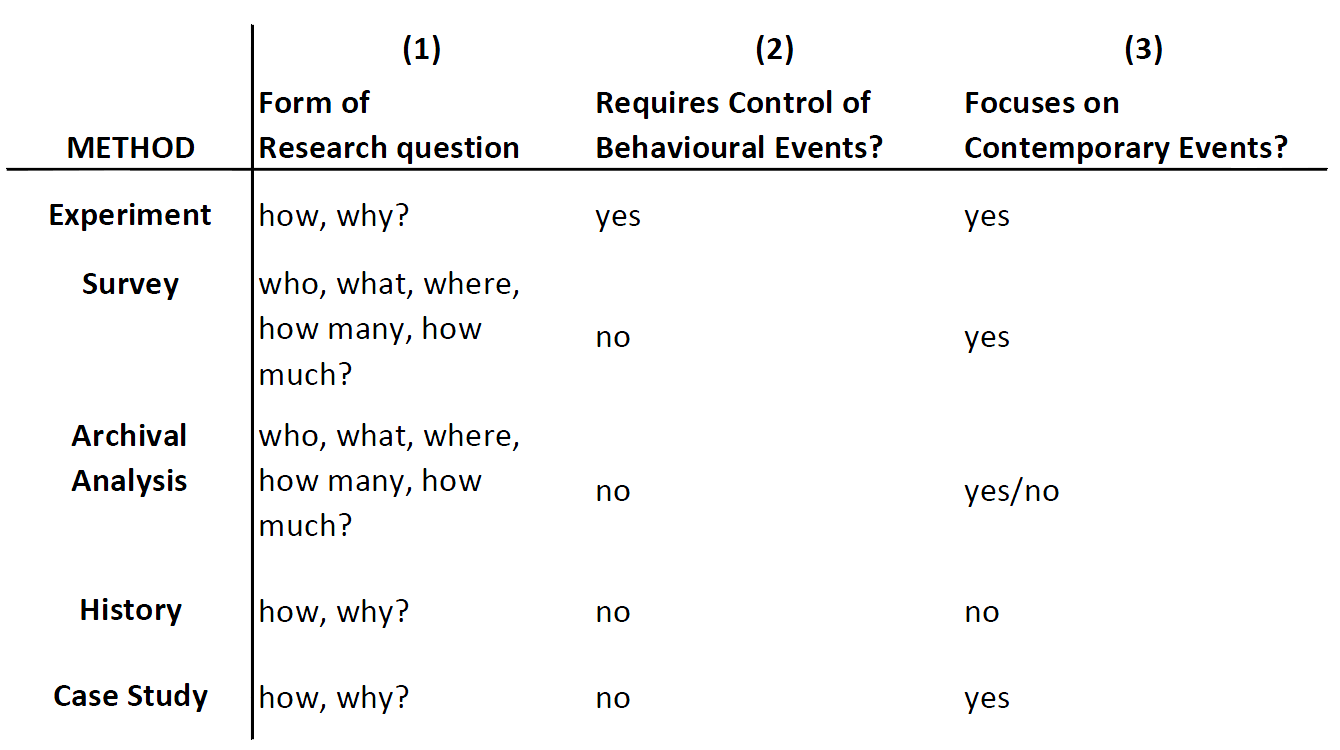
\includegraphics[scale=0.35]{methods.png}
\caption[Situations for different research methods]{Situations for different research methods, modified from \cite{CaseStudyResearch}}
\label{fig:methods}
\end{center}
\end{figure}

A case study is applicable to real-world projects, which is what we wanted to study. Another important advantage is that it can deal with various kinds of evidence, such as documents, archival records, interviews and artefacts.

\section{Qualitative research}
\label{sec:qualitativeresearch}
We used a qualitative research method based on relatively few informants. Unlike a quantitative approach where using questionnaires to gather information from a large number of participants is common, we wanted in-depth information from selected organizations. Using a qualitative research method enabled us to do rich and detailed analysis. 

The use of a quantitative method would have made statistical generalization possible, but it would have been more difficult to gather in-depth information. A survey may be easier to ignore, than a request for a face-to-face interview and a quantitative approach may not have given answers from the type of organizations we wanted. It may additionally be easier to get sincere answers in a face-to-face interview. In an interview the possibility to explain the questions is there. This is not the case for a survey, and it can be difficult to construct unambiguous questions that give good data for the analysis.

Further, we followed an inductive research approach. Deductive and inductive research methods are defined as follows\cite{bhattacherjee2012social}: 

\textbf{Deductive research:} The objective is to test a theory or hypothesis using new empirical data. This approach is known as \emph{theory-testing} research.

\textbf{Inductive research:} The objective is to infer theories and patterns from observed data. Also called \emph{theory-building} research.

In inductive research, researchers perform field studies followed by deriving theories from observations. This method is a contrast to deductive research where a theory is developed initially, followed by observations to evaluate it\cite{oates2005researching}.

\section{Case Study}
\label{sec:caseStudy}
This section describes case study as the chosen research method for this thesis. The content is derived from \cite{CaseStudyResearch} where Yin defines a case study in the following way:

\paragraph{Case Study:} An empirical inquiry that investigates a contemporary phenomenon in depth and within its real-life context.

%\begin{itemize}
%\item A case study is an empirical inquiry that investigates a contemporary phenomenon in depth and within its real-life context, especially when
%\item the boundaries between a phenomenon and context are not clearly evident.
%\end{itemize}
%\item The case study inquiry
%\begin{itemize}
%\item copes with the technically distinctive situation in which there will be many more variables of interest than data points, and as one result
%Hva er variables og hva er data points?
%\item relies on multiple sources of evidence, with data needing to converge in a triangulating fashion, and as another result
%\item benefits from the prior development of theoretical propositions to guide data collection and analysis.
%\end{itemize}
%\end{enumerate}

The case study inquiry relies on multiple sources of evidence and benefits from the prior development of theoretical propositions to guide data collection and analysis.

The research process is illustrated in figure \ref{fig:caseProcess}. As the figure shows, the process in linear, but iterative. This means that one can go back to previous phases if needed. The Plan phase consisted of identifying research questions and deciding to use case study as the research method for this study. The Design phase is about getting from initial questions to conclusions or answers. It is the logic that links the data to be collected to the initial questions of the study. 

\begin{figure}[h]
\begin{center}
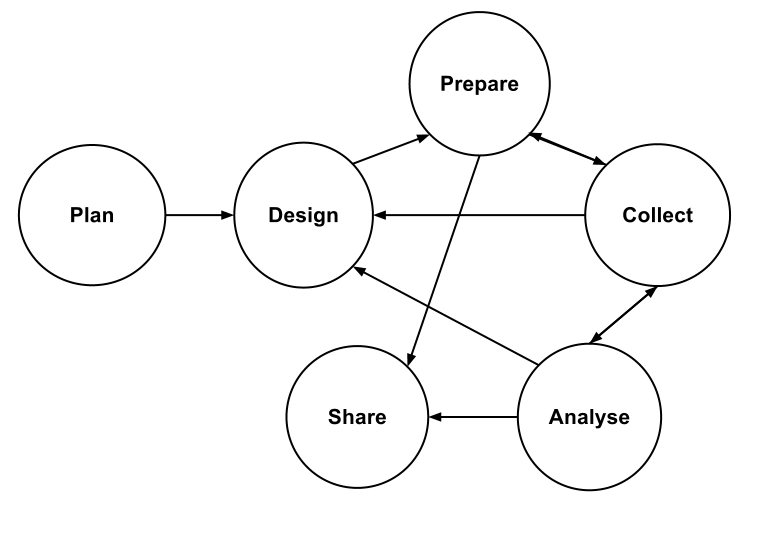
\includegraphics[scale=0.38]{caseProcess.png}
\caption[Case Study Research Process]{Case Study Research Process \cite{CaseStudyResearch}}
\label{fig:caseProcess}
\end{center}
\end{figure}

Yin presents tactics to maximize the quality of empirical research. He recommends to use multiple sources of evidence and to have key informants review a draft of the report. Both of these tactics were used in this study. 

The choice between a single- and multiple-case belongs to the Design phase. Multiple-case is usually preferred and was chosen as the method for this study. Additionally each case may be embedded or holistic. An embedded case has more than one unit of analysis. The design for this study is a mix. It is a multiple-case study where one case has three embedded units of analysis and two cases are holistic. The design of our study is illustrated in figure \ref{fig:caseDesign}.

\begin{figure}[ht]
\hspace{-0.28cm}\includegraphics[scale=0.375]{caseStructure.png}
\caption[Case Design for This Study]{Case Study Design, modified from \cite{CaseStudyResearch}}
\label{fig:caseDesign}
\end{figure}

The Preparation phase was very important as we did not have experience with the case study research method. The main activities performed in this phase were acquiring desired skills to become case study investigators and preparing for the specific case studies. It is considered difficult to obtain these skills as procedures are not routinised. It is advised to prepare to ask good questions, be a good ``listener", be adaptive and flexible, have a firm grasp of the issues being studied and be unbiased by preconceived notions. We have performed a background study in order to get a thorough understanding of the issues in the study. Relevant background information is discussed in chapter \ref{chp:background} and the background study itself is briefly discussed in section \ref{sec:background}. %Develop a protocol for the investigation? screen candidate cases? Pilot case? No..

Interviews, documents and surveys were chosen as the sources of information in the Collection phase. The use of multiple sources of evidence is consistent with the definition of a case study, which is presented in the beginning of this section. The interview is seen as being one of the most important sources of information in a case study. Documentary information is likely to be relevant in any case study. These data collection methods are described and discussed in sections \ref{sec:interviews}, \ref{sec:documentStudy} and \ref{sec:employeeSurveys}.

The Analyse phase is described in section \ref{sec:qualitativeAnalysis}.

The Share phase consisted of preparing, writing and editing this report. Choices such as to anonymize identities of individuals and individual organizations were part of this phase. This choice is further discussed in section \ref{sec:ethical}. It was a choice that was made as part of the preparation of the study and this illustrates the arrow from Prepare directly to Share, and shows that the case study process is not purely linear. 

\subsection{Background Study}
\label{sec:background}
The first step in our research were a background study of security incident management. In order to find appropriate questions for the interviews we found it necessary to study relevant literature such as standards and best practice guidelines. We focused on the well-established and internationally accepted ISO/IEC standards and documentation from the \ac{NIST} as well as various other guides.

We also looked at related work and what has been studied earlier in the field of incident management. In this way the background study was used to guide the data collection. It was also used in the data analysis, by comparing standards and prior developed theory to the findings of this study. This is consistent with the definition of a case study, as presented at the beginning of section \ref{sec:caseStudy}.

\subsection{Qualitative Interviews}
\label{sec:interviews}
We chose to perform qualitative interviews in our research as they are well-known and powerful tools for information gathering in qualitative research\cite{myers2007qualitative}. The main objective of qualitative interviews is to see the research topic from interviewee's perspective and understand why and how they got that particular perspective\cite{cassell2004essential}. To meet this objective, qualitative interviews are driven by open questions, a low degree of structure and often focus on specific situations and experiences made by the interviewee. 

We used what is referred to in literature as semi-structured interviews\cite{cassell2004essential}. We wanted interviewees to talk freely about their experiences, and thus we did not follow a strict order of predefined questions. However, to ensure we got all necessary information we used an interview guide. The interview guide worked as an incomplete script and states the main goals for our research as well as the main research questions and topics for the interview. The interview guide can be found in Appendix B.

Questions were not asked in any pre-defined order during interviews. This enabled us to ask follow-up questions and ask for elaborations on certain topics. When using semi-structured interviews, interviewees can be seen as being ``participants" in the research, rather than objects only answering pre-defined questions.

Interviews were performed face-to-face and voice recorded. We believe that conducting interviews face-to-face helped build trust with interviewees and thus gave better and more elaborative answers. It also gave us opportunity to explain and elaborate questions that were unclear. Since we recorded all of the interviews we could focus on listening and thus ask valuable follow-up questions instead of being distracted by writing down answers. Additionally, we could listen to the recordings several times as needed and clarify things that were unclear later.

%Developing an interview guide, carrying out interviews and analysing them can be highly time-consuming activities. Participating in interviews is also time-consuming for interviewees, which could have made it challenging to recruit interviewees for our study. One mitigation to the risk of not recruiting interviewees was sending out letters explaining the main purpose of our research, what was expected by the interviewee, and how the interviews would play out. We also notified organizations at an early stage and set dates for the interviews to ensure their commitment.

%Qualitative interviews are very flexible as they can be used to tackle various forms of research questions related to organizations. Despite the time effort spent on developing an interview guide, questions and conducting interviews, we found qualitative interviews to add great value to our research.

\subsection{Document Study}
\label{sec:documentStudy}
In case studies, documents are often used to verify or to question data obtained from other data collecting methods. To complement information gathered from interviews we studied relevant academic literature, standards and organization-specific documents such as policies and plans. This enabled us to compare standards, plans and current practice of incident management in organizations.

When using documents in research one should be aware of possible bias and other elements that could compromise reliability\cite{oates2005researching}. In our case study we looked at both public and confidential documents.  We believe that by signing confidentiality agreements we were presented with authentic documents from participating organizations. Nevertheless, we kept in mind that information could be outdated, not applicable or incorrect.      

\subsection{Employee Surveys}
\label{sec:employeeSurveys}
By studying documents and performing detailed interviews we got a thorough knowledge about routines related to incident handling. We found it interesting to examine how well these routines were established among the employees in the various organizations. To accomplish this we developed a list containing five main questions. These were asked to randomly selected employees without any specific background in IT. The questions can be found in Appendix C.
 
%\section{Action Research}

\subsection{Qualitative Data Analysis}
\label{sec:qualitativeAnalysis}
As discussed in \ref{sec:qualitativeresearch} we have chosen a qualitative and inductive research method. For the data analysis we used a ``general inductive approach", as described in \cite{thomas2006general}. In this article, David R. Thomas presents a ``systematic set of procedures for analysing qualitative data" and explains a ``straightforward approach for deriving findings in the context of focused evaluation questions". We found this approach to be less complicated and more suitable than other approaches to qualitative data analysis such as grounded theory, phenomenology and ethnography research approaches\cite{thorne2000data}.

Inductive analysis is often guided by predefined research objectives. The use of research questions as guidance in data analysis will undoubtedly set constraints on the number of possible interpretations and outcomes as it draws attention to specific aspects of the data. However, by using the general inductive approach rather than a stricter and more structured methodology, we believe it enabled findings to emerge from themes inherent in the raw data despite the pre-set research questions. Also, by using this approach, findings were not restricted by the methodology used. 

As a first step in our analysis we perused the data and identified themes and categories found related to our research questions. The process from raw data to main findings and conclusion can be outlined as follows:
\begin{enumerate}
\vspace{0,5cm}
\item Detailed readings of the qualitative data
\item Identifying specific themes that captured core messages given by participants.
\item Grouped themes into broader categories with corresponding labels and descriptions.
\item Primary findings are represented as a framework of themes.
\vspace{0,5cm}
\end{enumerate}

Using this method for analysis enabled us to meet the main objectives of inductive research which are; to compress the qualitative data into a summary format, to establish links between research objectives and findings and to develop theories or models about the underlying structure of experience found in the data\cite{thomas2006general}. The outcome of an inductive analysis is thus typically a model or framework holding categories or themes that summarize the raw data. Unlike the grounded theory methodology, ``researchers using the general inductive approach typically limit their theory building to the presentation and description of the most important categories"\cite{thomas2006general}.

To verify the credibility of our findings we provided a summary of the relevant interview to participants. They were thereby given the opportunity to challenge our interpretations and comment on whether our findings were in compliance with their personal experience.

Using this approach for data analysis, our main findings derive from both our predefined research questions as well as from findings arising directly from the data through multiple readings and interpretations. 

\section{Participants}
%In the nature of qualitative research participants were chosen to be diverse such that different perspectives on incident management (in the same context) could be studied.large organizations that are likely to have experiences severe security incidents. + de i Gjovik gjorde paa small/medium.. her gjor vi en dybdestudie av noe annet!Hvorfor de vi valgte? Hvorfor er de interessante? 
The participating organizations in this study are all large organizations. The core activities of the organizations belong to fields defined by organizations like \acs{NSM} to be extra exposed to attacks. This could indicate that they are experienced and well equipped to handle information security incidents. We found it interesting to examine how such assumed experienced organizations perform incident management and what challenges they face. Additionally the participating organizations have quite different organizational structures, which could also lead to interesting findings.

\section{Ethical Considerations}
\label{sec:ethical}
%Litt i forhold til at man behandler sensitiv information og saann
The main ethical concern related to our research is the potentially confidential information revealed during interviews. It is unlikely that organizations want details about their information security practices to be publicly known. Another important aspect was that we performed interviews and the privacy of the participants had to be considered. Since a voice recorder was used during interviews, participants could potentially be identified later by voice recognition. To make sure that the participants knew exactly what they participated in, they were given information about how collected data was handled through a statement of consent. They were also given the right to withdraw from the study at any given time. This project was reported to the Norwegian Social Science Data services. The information sheet, including the statement of consent can be found in Appendix A (in Norwegian). Before submitting the report, the participants were given the opportunity to read through the material and correct any potential misunderstandings.   

As we got insight into confidential documents, we had to sign confidentiality statements beforehand.


\subsection{Anonymization}
No individuals or individual organizations are recognizable in this report. Participating organizations are given pseudonyms. All relations between individuals and individual organizations and results are anonymized at the end of the study, and only available to the students and partly their supervisors during the study. The term anonymization means that any information that could directly identify individuals or individual organizations is deleted and that any information that indirectly could identify individuals or individual organizations is deleted or changed. At the end of the study all recordings are deleted.

\section{Challenges}
This case study relies on qualitative information and a challenge related to that is to work hard to report all evidence fairly. Additionally this type of research provides little basis for scientific generalization. \cite{CaseStudyResearch}

For quantitative data there exist clear convention for analysis, but there are fewer guidelines for the analysis of quantitative data. In relation to this Allen S. Lee states in \cite{lee1989scientific}, ``but the analyst faced with a bank of qualitative data has very few guidelines for protection against self delusion".

Basing most of our information gathering on interviews, the challenges with this approach had to be carefully considered. The authors had little or no experience in preparing and conducting qualitative interviews. Michael D. Myers and Michael Newman discusses potential challenges with using qualitative interviews in\cite{myers2007qualitative}. 

They mention the artificiality of qualitative interviews where one interrogates a stranger that does not know or trust you. The lack of trust may cause the interviewee to withhold information that could be of value to the study. As an attempt to mitigate trust issues the procedure of handling data (anonymization) was presented as well as highlighting that the project had been reported to the Norwegian Social Science Data Services.   

Problems could also arise if too little time is assigned for the interviews. Questions could be rushed causing inaccurate information or that important information are left out. To avoid time limitations being a concern, we assigned more time than estimated for each interview. We also used the interview guide with predefined questions and topics as well as correcting any misunderstandings during the interview to avoid ambiguous questions.

When relying on qualitative interviews for information, one have to consider potential interviewee bias as for instance security incident management knowledge vary greatly among employees in an organization. In addition, Myers and Newman mentions the possibility for interviewees to construct knowledge to appear knowledgeable and rational. By giving interviewees enough time to answer questions and carry out interviews as a dialogue, we hope to have avoided these problem.

One challenge of using qualitative data is that interpretation of information is somewhat based on researchers' background. Being students with similar backgrounds and limited experience we believe that choosing an inductive qualitative research approach gave less bias in our results since we did not aim at proving a specific theory, but rather aimed at starting our information gathering with open minds. 

A challenge related to empirical research is that it relies on other people. We experienced that it was at times difficult to make contact with people and this led to at times slower progress than desired.

The interpretation of data is based on researchers background.



\cleardoublepage
\chapter{Case Introductions}
\label{chp:CaseIntroductions}
This chapter gives an introduction to the specific cases studied in this thesis. The study contains three separate cases where a different organization is studied in each case. All of the organizations are classified as large organizations. In Norway an organization is large if it has more than 100 employees \cite{SMB}.

\section{Case A}
This organization is a large Norwegian government-owned organization. They have 200 employees that work with IT, and a larger number of users of their systems. The interviewee is the IT security manager. His responsibilities include both technical and more administrative tasks. He has had this role for about two years.

The organization handles most of its own IT operations. Some services are outsourced, but they mainly handle the IT operations themselves. They have an IT-manager with a staff that includes the IT security manager. They have a customer service center %eller service deks eller noe? 
that handles user support and receives cases from users when something happens. The organization also has a network section that is responsible for ensuring that their network infrastructure works as intended. Additionally they have  a section that operates their servers. They have large systems, like a system for email and a system for handling employee and user data. They also have a section that handles their applications. This includes both developing, maintaining and operating their applications.

\section{Case B}
The Norwegian organization in this case is a large, independent and non-commercial organization with a couple of thousand employees. They possess large amounts of valuable and sensitive information and information security is thus a high priority in their business operations. The two interviewees in this case are the IT- and IT-security manager and the Supply manager, both working in the IT-department. They have had these roles for four and six years respectively. They deliver IT-support for all the organization's departments and are involved in incident management regularly.   

In addition to the IT-department, that is responsible for all shared IT-services in the organization, IT is organized further hierarchically such that each individual department has their own IT-manager responsible for local IT-support concerning their department. The IT-managers are also responsible for information security within their departments.

The organization has to a large extent outsourced their IT-operations and has    many suppliers. The main IT-operations are delivered by one external organization, whereas application operations are delivered by an external consortium. These two main suppliers of IT-operations are referred to as supplier 1 and 2 in this report. These two are the main suppliers of IT-operations, however there are others as well. 

%skrive noe om supplier 1 og 2 her kanskje?

\section{Case C}
This organization is a large Norwegian organization with several thousand employees. They deliver IT-services to customers in addition to operating their own infrastructure. The interviewee is the IT security manager  and the operational leader of a department that is responsible for security, quality, compliance and risk. He has had this role for about two years.

In such a large organization, departments have different requirements for security and thus various policies are implemented throughout the organization. In addition to operating their own incident management, they are also responsible incidents concerning services they deliver to customers. Consequently, the organization deals with security incidents on a daily basis. In addition to dedicated incident managers, the organization has its own \ac{IRT} to assist in major incidents. The \ac{IRT} also handles incoming notifications from internal users regarding security issues and may also deal with incidents concerning customers. 
\cleardoublepage
\chapter{Findings}
\label{chp:findings}
This chapter presents findings from the document studies and interviews. The findings from each case are described separately. It should be noted that in this chapter, information has not been analysed or interpreted by the authors, but only introduced as given in the interviews or found in the documents. The \textit{grouping} of the information however, is based on the standards and guidelines presented in section \ref{section:standardsandguidelines} and represents the first step of the qualitative data analysis approach, as presented in section \ref{sec:qualitativeAnalysis}. 

\section{Case A}
This section describes the results from interviews and document study for Case A. 

\subsection{Preparation}
The IT security manager defines an incident %Skal endre dette til information security? Han nevnte at det ikke trengte å være IT-relatert engang, så kanskje ok å bare skrive incident?
as the occurrence of something unwanted. This includes both occurrences belonging to a predefined category of unwanted incidents and occurrences of a nature that you see is unwanted. More specifically an \ac{ICT} incident will usually involve loss of information or loss of control over information systems. This is a definition that is known in the organization. The categories of unwanted incidents are determined through risk assessments. It is stated in their principles for information security that they have to perform risk assessments and this document is approved by the management and distributed to all parts of the organization. Their information security policy refers to this document. Several of the principles address risk management. They have another document that further specifies their risk assessment process. %Se prinsipper for informasjonssikkerhet del 1, referer videre til rutiner for risiko og sårbarhetsanalyse

The IT security manager points out loss of information related to the organization's core activities to be the worst information security incident they can experience. This could damage their relationship to partners, their general reputation and their credibility. Additionally it may damage the work and career of individuals with ownership of the information. %Gir dette bort for mye info?
Another aspect is that they own information that should not fall into the wrong hands. This can be information that goes under the \ac{UN} treaty on the non-proliferation of nuclear weapons (NPT) \cite{NPT}, which includes information that may be used for spreading of nuclear weapons and weapons technology. %Er dette ok å skrive??
The loss of such information could obviously have severe consequences.

The organization has, as mentioned, an information security policy and a principles for information security document. The latter is to be updated if there are changes in the threat landscape or at least every other year. It is currently a subject for audit. It is up to each department to make sure that employees and other users are aware of these documents. The IT security manager does not expect that all of the users have detailed knowledge of these documents, even though it is stated that all users have to comply with them. The IT department uses these documents actively. %NB spør om dette i ansatteinetrvju!!!
During the last years the level of threat has increased for this organization and as a consequence they are going to perform a risk and vulnerability assessment for all the departments in the organization. In addition to the mentioned documents, they have an internal policy for incident handling.

They have several systems that are critical for their operations. This means that they need backup solutions for these systems in case of incidents. The IT security manager thinks that they have very good continuity plans. They have among other things tried to avoid any single point of failure to increase redundancy.

They have an information department that is responsible for all external communication and they cooperate closely with the IT department. The organization has a procedure for contact with the police in case of any violation of law. If the organization wishes to report a crime it is the manager that has to do this, although the IT security manager will provide the police with any relevant information he has access to. The manager is the only one that can report crimes on behalf of the organization, as this is a government owed organization.

They do not have a holistic plan for incident handling because no incidents are the same. Related to that he stated:

\begin{quote}
\textit{``To have a detailed guideline that takes all possibilities into account and that you have to change each time you get a new system %. I think that would be 
[...] we are not that good [...] and I don't think we have ambitions to be that good either"}
\end{quote}

They do however have general guidelines for handling of security incidents. Certain types of incidents are repeating, like phishing, and they have more detailed guidelines for these specific types of incidents.

If a system owner discovers a vulnerability in his system he will notify the IT security manager about it and about the scheduled update for the patch. The process is the same if the system owner is generally not satisfied with the security of the system.

\paragraph{\acl{IRT}}
Because the organization has an internet domain they are required to have an abuse email-address and they have a team that is responsible for receiving and handling cases reported to this address. Some of the members of the abuse team are part of the IT-support function of the organization and are part-time employees. Cases that involve employees, botnets or spam are handled by full-time employees at the service desk. One of the full-time employees is the leader of the team. The IT security manager is also part of this team in a supervising role. The team consists of seven people. The cases sent to abuse are not just received on an email address, but go straight into a case management system. Incident handlers are required to give the reporter an answer so that he knows that the potential incident is being looked into and that his report is appreciated.

The usual notifications will be received during work-hours, but they also have someone available 24/7 if something extra serious occurs. In that case they need to be alerted specifically, and it will typically be a system owner who will notify the person on duty.

They have a tool for mapping IP-addresses to users at specific times, that they need to use related to incidents. There is one person in the team that is responsible for this tool. They also have someone responsible for administrative tasks such as shifts. There is additionally someone who is responsible for documentation, especially in cases they have not seen before.

The team performs a limited amount of preventive work. They see repeating incidents and have reviews of larger incidents and use this to identify changes that are needed. They use the \ac{ITIL} framework, discussed in section \ref{section:ITIL} of this report, and treat repeating incidents as problems.

They often need to communicate with the various sections of the organization when incidents occur. The people working there are not specialized in handling security incidents, but they know how the systems work, and are therefore important resources. There is a daily designated contact person for some of the sections. The IT security manager mentioned that this communication can be challenging, especially for the sections that do not have a permanent designated contact person. Last year they experienced a targeted phishing attack and this led them to gather a team consisting of resources from various sections.

Most of their employees involved in incident handling have an IT background and thereby a solid technological knowledge. Additionally they go through a training process when they are hired. There is also a thorough interview process. During their time in the job they often get new tasks and need training for this.

\paragraph{Standards and Guidelines}
The organization uses \acs{ISO}/\acs{IEC} 27001 and 27002, but they do not aim to be certified. Their information security policy states that they are to be in compliance with these standards. The IT security manager thinks that a certification would be useful, because the most important part of the certification is the commitment of the management related to the standard. Because they are a government owned organization they are required to use \acs{ISO} standards. This is a relatively new requirement and he sees it as being one step closer to a certification.

The organization has reviews of incidents and uses this to make changes in their \ac{ISMS}. They also use \ac{ITIL} in their security work and incident handling. They do not use all recommendations from \acs{ISO}/\acs{IEC} 27001 and 27002 and \ac{ITIL}, but choose the parts they see relevant for their organization. The IT security manager is somewhat familiar with \acs{ISO}/\acs{IEC} 27035, but the standard is not implemented in the organization.

\paragraph{Awareness and Training}
The organization conducted an information campaign with an external supplier about a year and a half ago. The supplier delivered slides containing small lectures that were sent via email. These were lectures about themes such as how to protect your password. In relation to their attitude towards awareness, he stated: 

\begin{quote}
\textit{``There is a principle that says, never waste a good crisis"}
\end{quote}

This means that they use incidents, typically that others have experienced and communicate these to the organization. He mentioned that personally he takes any opportunity to talk about the importance of protecting information.

The IT security manager thinks that their classification of information is not satisfying. He thinks that users are not aware that the information security policy states that they have to classify the information they process. This highlights that the policy needs to be better established in the organization. This is the managers responsibility and he emphasizes again that a more extensive use of \acs{ISO}/\acs{IEC} 27001 and 27002 could help as this would lead to increased management commitment.

About a year ago they conducted a contingency rehearsal with information security as the chosen theme. The management was involved in this training. It included seven levels of escalation. The training contributed to increased information security awareness in the management as well as being a test of their central contingency plan.

He thinks that you will always benefit from rehearsal. Everything he can use to increase management awareness related to information security is beneficial. It is however challenging to conduct rehearsals and he stated:

\begin{quote}
\textit{``The most important part of preparing a rehearsal is to make sure that the responsible people train on the right things and to create a good and relevant game that challenges the involved people and that they feel is realistic [...] That is the most important thing, to give them what they need in order to be able to handle a real situation."}
\end{quote}

They use their risk and vulnerability assessments to determine what to focus on in rehearsals. The use rehearsals both for situations where they already have routines and for situations where they do not yet have any. A rehearsal may identify what routines they should have.

He says that they have many examples of issues that have been revealed through rehearsals. One such example is that even though various employees may have a certain risk awareness they may not agree on what the actual risk is. They have planned rehearsals this year as well, where one is to be conducted in cooperation with a partner organization. %Heter det oartner organization?

\subsection{Detection and Analysis}
The organization uses several means for detection of information security incidents.

\paragraph{Initial Detection}
%Ta med rapporteringsrutiner og ansattes kjennskap til disse her??
Incidents can be reported via the abuse system, as described in the \ac{IRT} paragraph. Additionally their internet supplier notifies them if they see that there are any compromised hosts in their network. They can also assist in the incident handling upon request.

The organization has a relatively new deviation management system. This system can be used to report various types of deviations, from information security to \ac{HSE} related deviations. It does not necessarily have to be an incident, but it can be any type of deviation, such as a vulnerability. It is mainly used for internal cases, and thus differs from the abuse system. The IT security manager hopes that this system will be used more for information security related incidents than it is today. This system also works as a database of incidents, as it includes information about all reported incidents (in the system).  

They have a tool that can be used to monitor connections to their network. This can be a source for incident detection.

The IT security manager thinks that they have underreporting but that people in the organization are good at reporting things like suspicious emails. He does however think that they are not good at reporting the extent to which they have actually disclosed any sensitive informations. He says that this originates in establishment of attitude and training. He states that:

\begin{quote}
\textit{``Users of a system need to understand what possibilities there are in the system, but also what limitations there are."} 
\end{quote}

\paragraph{Categorization}
The organizations categorizes incidents based on type (spam, phishing, botnet etc.) and based on what service or system they belong to. Incidents reported in their deviation management system are categorized based on whether they are \ac{HSE}-related technical or of other types. The category information security does not currently exist in the system, but it is planned to be included.

They also categorize incidents based on impact. They use the categories low, medium and high. Medium is when service is unavailable for several persons and high is when service is unavailable for the whole organization. Other incidents are categorized as low. The assigned impact category sets a time limit for how fast the incident must be resolved.

\subsection{Incident Response}
Cases reported to abuse are categorized and dispatched to the second line of incident response. %hmm, litt usikker på hva akkurat det betyr
From that point it is either resolved or transferred to another section, such as the network section, if they are better equipped to handle it. It can also be solved in cooperation between incident handlers and employees from other sections.

The IT security manager is not very concerned about getting systems up and running as fast as possible after an incident. This is because he wants to make sure that that the incident is properly resolved. There have been cases where he wanted to perform risk and vulnerability assessment of systems, but has not been allowed to do so.

After an incident the system owner is asked to identify what has been lost or compromised. It is also their job to try to assess if the organization has suffered an economic loss. They do know that they have used employee time on the incident, but other factors, such as the value of information, are hard to estimate. The IT security manager wishes to work on value assessment of information. He wants to do this by asking the owners of information.

If an incident is serious it will be reported to the management. The IT manager is notified about larger incident, but not small routine cases.

An example where the IT security manager used their network monitoring tool, he discovered that several users logged in on the same foreign IP-address. He then contacted them and found that they were in fact abroad, and that their user accounts had not been compromised. By contacting them first the users avoided a cumbersome process of being blocked and having to regain access. The organization also has tools that they use to analyse emails in spam cases. They have the possibility to log in to the email server as admin and fetch emails sent to people. This is only done in serious cases, and if it is done, they only look at emails relevant to the case in order to maintain privacy. The IT security manager has only done this once, in relation to a targeted phishing attack. This attack happened in two stages where the first stage was targeted to the organization and was used to retrieve usernames and passwords from users. The compromised user accounts were subsequently used to send new bank-phishing emails.

\begin{figure}[H]
\hspace{-1.1cm}
\includegraphics[scale=0.53]{WorkflowCaseABotnet.png}
\caption[Workflow for a Botnet Incident, Case B]{Workflow for a Botnet Incident}
\label{fig:WorkflowCaseABotnet}
\end{figure}

\paragraph{Workflow}
The organization has specified workflows for specific types of incidents. They do not have a general workflow that applies for all incidents. Figure \ref{fig:WorkflowCaseABotnet} illustrates the workflow for a botnet incident. The figure is derived from a description given at the interview. 

\begin{itemize}\itemsep-0.2cm
\item The process is initiated by a report received in their abuse system or from some other source. 
\item The incident is categorized based on type (botnet, virus etc.)
\item If there is more than one affected host, the case will be split into one case per host and the following steps will be taken for each case.
\item If the incident is particularly serious the host will be blocked and the user in question will subsequently be contacted.
\item If the incident is not so serious the user in question will be contacted and subsequently blocked.
\item If contact is not established the user will be blocked and then tried contacted again.
\item The affected host is cleaned up.
\item The user will regain access.
\end{itemize}

\paragraph{Escalation}
They have a contingency plan for the IT department, that describes a set of incidents. This plan is initiated if an incident is particularly serious. It does not directly target information security incidents, but it includes scenarios where systems are unavailable. A system is unavailable if they have lost control over either if someone has taken control over the system or if there has been unauthorized access. The loss of admin passwords is an example of such an incident. When there is an incident so serious that the contingency plan must be initiated the management is also involved. The contingency plan includes communication routines related to incidents. 

\paragraph{Electronic Evidence}
They have good cooperation with the police and in cases that may lead to criminal cases they do not try to investigate themselves, so that they will not destroy any evidence. If they suspect criminal activity they contact the police and do nothing else themselves prior to this contact. They do however block users upon request from the police, in order to preserve evidence.

When it comes to accessing user-owned files they follow the Norwegian Personal Data Act.

\subsection{Lessons Learned}
The IT security manager thinks that their routines usually work well. When they have not worked well there is a review of the incident.

An example of an incident that was handled well is an incident that happened after they implemented storage for the entire organization. The OS they used had a default configuration where ports were left open. This was not something they had paid much attention to before implementing their solution. There turned out to be a vulnerability in this OS that someone was able to exploit. This led to the organization being used to enhance a \ac{DDoS} attack. This was detected and reported by email. They saw that one host had several millions unique external connections during 24 hours. They contacted the user in question  and involved the network section to find out what was going on. The were able to reveal that there had been no unauthorized access to the storage system itself, but only to the OS used.

The IT security manager points to lack of staff  both in general and dedicated to information security as well as lack of routines as challenges related to information security incident handling in their organization: 

\begin{quote}
\textit{``I would rather say that it is perhaps too often that we have incidents where we do not have routines that are sufficiently described. %(godt nok beskreve rutiner)
As I said earlier, you cannot have routines for everything, but I also think it originates in the organization and how we are staffed to handle situations. There is no point in writing routines that do not establish ownership to a process [...] For example we have routines for handling a botnet incident, and these two cases were dispatched this morning and no-one has addressed them yet."}
\end{quote}

As a general statement he said: 

\begin{quote}
\textit{``There is always room for improvement"}
\end{quote}

The IT security manager gathers information about information security incidents and creates annual reports to the management. This way they have an overview over previous incidents. They do not evaluate absolutely all incidents as this would be too much work. It turns out that lack of awareness among users is often the root cause of incidents. The ``solution" to these incidents is therefore awareness-raising activities rather than changes in routines.

They have a process they call review. This includes processes and people and not only technical details. They have reviews for incidents of a certain scope and when they experience that their process is not efficient enough or clear enough. The IT security manager is satisfied with their review process. Necessary identified improvements have been implemented and identified mistakes are not repeated.

They have exchanged information and experiences with both \acs{NorCERT} and other \acp{CERT} in relation to specific incidents.


\section{Case B}
\subsection{Preparation}
\paragraph{\acl{IRT}}
\paragraph{Standards and Guidelines}
\paragraph{Awareness and Training}
\subsection{Detection and Analysis}
\paragraph{Initial Detection}
\paragraph{Categorization}
\subsection{Incident Response}
\paragraph{Workflow}
\paragraph{Escalation}
\paragraph{Electronic Evidence}
\subsection{Lessons Learned}

\section{Case C}
This section describes the results from interviews and document study for Case C.

\subsection{Preparation}
The organization has several internal departments. They use different incident handling plans depending on the type of security incidents they are dealing with since various expertise areas are required to respond effectively. 

The organization has implemented several measures to prepare for security incidents. They have developed three frameworks for incident management where each framework addresses a specific category of incidents. These frameworks describe relevant roles and activities for handling the organization's three main categories of incidents:

\begin{itemize}
\item IT operational-related incidents (service interruption etc.)
\item Information security incidents (breach of confidentiality, integrity and in some cases availability (such as DDOS attacks))
\item All other incidents (terror, accidents etc.)
\end{itemize}
 
Even though the IT security manager describes an incident as being loss of information, other events such as DDOS attacks are also defined as incidents even though it is the availability of information that is compromised rather than confidentiality or integrity. In most cases he thinks of security incidents whenever there is an attacker trying to steal information. Nevertheless, he highlights:

\begin{quote}
\textit{``90-95\% of the security incidents we experience are availability related incidents"}
\end{quote} 
 
It is essential for the organization that customers trust them and their services. The IT security manager identified loss of sensitive customer information, service unavailability and other incidents that could possibly lead to a weakening of the trust relationship as the most serious consequences of information security incidents. 

The organization's security policy aims to communicate the management's direction and commitment to information security. One of the main objectives stated in their security policy is that information security should be part of their risk management and long-term strategy. Information security should be revised, improved and sufficient resources should be allocated. The policy states that it is the management that has the ultimate information security responsibility, but that their success relies on the collective effort of everyone involved, especially all their competent and dedicated employees. Information security is stated to be a critical business issue, and thus the organization strives to create a security-positive environment.

In addition to the top level security policy, there are different policies for each individual department as their need for security varies. Additionally, contingency plans are implemented and revised continuously. The organization has a predefined plan for communication with the media during major incidents. 

\paragraph{Awareness and Training}
The IT security manager mentioned that they perform extensive work to raise awareness related to security among employees. New employees participate in courses where they are introduced to the organization's security handbook and they have to sign that the content is known and understood. The security handbook is also revisited annually during employee appraisals where employees have to reconfirm that the content is known. In addition, employees are invited to lunches and security-related presentations regularly. The intention is to increase the overall competence and to ensure that security guidelines are read and not forgotten.

The organization does not conduct training for employees addressing the most common incidents. The IT security manager emphasized that their plans and procedures are being used so often in practice that there is no need to arrange training for these cases. However, in accordance with the ITIL framework the organization conducts rehearsals once a year with a scenario they believe is useful. The organization performs rehearsals in cooperation with customers regularly, as they often wish to include their IT service providers. Additionally, training in cooperation with the government takes place every other year. 

\subsection{Detection and Analysis}
There are several ways that incidents can be detected.
\paragraph{Initial Detection}
The initial detection of incidents can either be performed automatically by a server, triggered by an alarm or discovered manually. Often, network analysis have to be done manually to detect security breaches. Whenever employees experience something abnormal or unexpected they are advised to report it to the \ac{IRT}. Examples include emails from unknown senders or email attachments that do not work as intended. The attachments may fail to open or display something indicating that a script is being run for a few seconds.

The IT security manager suspects underreporting of incidents among employees. He believes the threshold for reporting is high and that employees often omit to report suspicious events. This could either be due to employees failing to see the importance of reporting incidents or that they do not want to acknowledge potential mistakes they made. The IT security manager says they would rather have too many events being reported than too few, and they therefore work continually to emphasize the importance of reporting incidents.

Security vulnerabilities are reported through a risk framework, where they are evaluated, categorized and potentially escalated. The organization does not operate with anonymization for employees that report security events, but codes of conduct says one could use an external law firm if someone wishes to report incidents anonymously. However, this opportunity has not been used by employees so far. 

\paragraph{Categorization}
The organization does not follow any standards for categorization. They categorize incidents as being of low, medium or high impact. Whenever incidents are handled they are linked to these levels and handled according to predefined procedures. An incident's impact level will determine what can be done in response. For high impact incidents, authorization is needed from customers in case systems need to be shut down or changes have to be made in the production environment. This represent complex incident responses and are referred to as emergency changes, but are in some cases necessary to mitigate serious consequences. 
The organization bases their categorization method on the ITIL framework, which stresses the importance of incident categorization. ``Accurate categorisation is important because it will allow useful metrics to be gathered highlighting areas of the infrastructure where incidents are occurring\cite{itilbok}." The organizations can use this information to improve exposed infrastructure and thus decrease the number of incidents over time.

\subsection{Incident Response}
The main purposes of incident response are to retain normal business operations, minimize business impact by ensuring service availability and to find a temporary solution to the causing problem. The IT security manager explains why keeping services up and running at all times are so important:

\begin{quote}
\textit{``Customers evaluate us as an IT service provider mainly on the availability of the services we deliver."}
\end{quote}
Thus, restoring service availability is a number one priority in the organization's incident response.

\paragraph{\acl{IRT}}
In addition to dedicated incident managers, the organization has its own \ac{IRT} to assist in major incidents. The \ac{IRT} also handles incoming notifications from internal users regarding security issues and may also deal with incidents concerning customers. Employees work day and night with ``normal business operations" and thus need security expertise available 24/7 in case of incidents. The \ac{IRT} works as a point of contact for the entire organization. They primarily assist in incident response and otherwise work as a pool of resources for incident managers. 

It is the incident managers that \emph{handle} incidents, whereas the \ac{IRT} assists with their expertise on security incidents. Additionally, the \ac{IRT} are granted certain mandates that allow them to shut down systems or acquire external expertise and assistance up to a predefined cost limit.    

The organization has their own \ac{IRT} handbook. The handbook aims to describe how the \ac{IRT} operates and is used to explain internal routines to new team members. The \ac{IRT} handles most of the organization's security incidents as well as some customers'. However, most customers have their own \ac{IRT}, although the organization offers their \ac{IRT} as a service for customers that do not have the capacity or need of their own team.

The \acp{IRT} communicate and coordinate with involved parties throughout the incident response. For critical incidents, a second team called the Critical Incident Management Team work as an internal support function for the \ac{IRT} and provides complementary competence. The two teams work together to resolve critical incidents. 

\paragraph{Standards and Guidelines}
The organization bases all of their service management processes on the ITIL framework discussed in section \ref{section:ITIL}. They follow the ISO/IEC 27001 standard, and have several certifications. Their incident management processes however, are mainly built on the ITIL framework. The IT security manager is not familiar with the ISO 27035 standard that addresses security incident management specifically. 

\paragraph{Workflow for incidents}
The workflow for incident management is based on the processes described in the ITIL framework. Figure \ref{fig:workflowcaseC} illustrates the workflow, which is derived from organization specific documentation as well as information given in the interview. 

\begin{figure}[H]
\hspace{-1.1cm}
\includegraphics[scale=0.49]{workflowcaseC.png}
\caption[Workflow for Incidents, Case C]{Workflow for Incidents}
\label{fig:workflowcaseC}
\end{figure}

\begin{itemize}
\item An incident is first detected or reported to the service desk.
\item Each incident is categorized and prioritized such that it can be handled correctly. Further, the service desk decides whether the reported event is truly an incident. In case of false alarms, the reported events are either rejected or handled as service requests.
\item The incident is diagnosed and possible negative effects are considered.
\item The service desk assesses whether the incident has a known solution and their capability to handle it.
\item Incidents with unknown solutions are sent to a group of specialists that conduct further investigations.
\item Escalating and severe incidents are passed on to the ``Major incident handling" process when appropriate. 
\item Once a solution is found, whether by the service desk or group of specialists, incidents are resolved.
\item The incident is fully documented with all relevant information.
\item The incident is closed and users confirm that the incident is fully resolved. 
\end{itemize}

\paragraph{Workflow for major incidents}
Major incidents are defined by ITIL as incidents of the highest and second highest priority. The organization has separate procedures for major incidents. Incidents in this category usually have a high degree of user impact and thus have higher urgency and shorter time intervals for response activities. These procedures are initiated in the ``Major incident handling process" whenever incidents are assessed as major. This is illustrated in figure \ref{fig:workflowcaseC}.  

Figure \ref{fig:workflowcaseCmajor} illustrates the workflow for major incidents. The content is based on organization specific documents as well as information given during the interview.

\begin{figure}[H]
\hspace{-1.1cm}
\includegraphics[scale=0.53]{WorkflowcaseCMAJOR.png}
\caption[Workflow for Major Incidents, Case C]{Workflow for Major Incidents}
\label{fig:workflowcaseCmajor}
\end{figure}

\begin{itemize}
\item When the organization handles major incidents, support in form of a Service Manager, Incident Manager or the Critical Incident Management team are engaged in the incident response.
\item It is evaluated whether an Incident Management Board is needed to handle the incident. If it is not, the incident is handled according to normal incident management procedures.
\item An Incident Management Board is established to ensure proper management and appropriate handling of the major incident. The \ac{IRT} may be part of the Incident Management Board whenever necessary.
\item If dedicated resources are needed, a Task Force is established. A Task Force is an ITIL term for a dedicated group of resources that are put together to solve a specific task.
\item When a solution is found, either by the Task Force or the Incident Management Board, the incident can be resolved.
\item The incident is documented and activities are logged.
\item The incident is closed and users have to confirm that it is fully resolved.
\item The incident is handed over to the Problem Management Process for further analysis.  
\end{itemize}


\paragraph{Escalation}
The organization has no predefined routines for escalation during incident response, even though they have done it several times in practice.

\paragraph{Electronic Evidence}
The organization has no in-house expertise on forensic analysis of electronic evidence. Mirroring disks for use as digital evidence approved for Norwegian courts is the only thing done by the organization itself with regards to electronic evidence. The analysis of the disks are done by an external third party or by the police.

\subsection{Lessons Learned}
The organization structures their learning process in accordance with the problem management process from ITIL. Improvements are identified during this process. 

After rehearsals a set of improvements are identified and summarized. Often, interaction with external parties are identified as areas of improvement, especially in accordance with customers. Collaboration and coordination across organizations and teams are proven to be challenging since different parts of incidents are handled by IT service providers and customers themselves. 

A centralized tool is used to document previous incidents in addition to experiences, potential improvements and internal audits. Meetings are held after major incidents where the incident response process is reviewed. Post-incident meetings are held by a problem manager who is responsible for the ITIL problem management process. Participants vary with the nature of the incident and the targeted environment. The IT security manager recognizes the benefits of post-incident meetings and stated:

\begin{quote}
\textit{``Often concrete measures are identified after incidents. Both organizational, process-related and on the investment side."}
\end{quote}

As an example he mentioned major DDOS attacks leading to customers investing in new equipment and new routines for communication being implemented. 

%Despite internal learning and review processes, experience and lessons learned are not often shared with external parties. How the organization perform incident management is not something they necessarily want to be public information as they wish to some extent to stay ``under the radar". Also, most often incidents occur with their customers and it is thus up to them whether information is shared. 

The IT manager explained why he thinks their routines work so well:

\begin{quote}
\textit{``Since we are such a large organization we deal with a large volume of security incidents and thus our frameworks work well. I believe it is much tougher for smaller organizations. If it has been years since the last incident it becomes more challenging to respond effectively."}
\end{quote}

The organization is currently working with a project for improving their incident management and so far it has proven to be very effective. It mainly involves improving quality in their many and complex value chains. The IT security manager described why this is important in incident management:

\begin{quote}
\textit{``One of the most important things with incident management is keeping track of and understanding value chains: which, when and how components are communicating."}
\end{quote}

Large organizations often have complex and long supply chains. Through the improvement project they identified weak quality in their value chain descriptions as a problem for effective incident response. The diagnostic work was complex, and sometimes it was challenging to identify what happened, where it happened and with what consequences. The organization has started extensive work to identify any single-point-of-failure and make value chains more robust. The project started in one of the organization's departments but quickly escalated to include larger parts of the organization as they saw positive results. The project's objective is to identify vulnerabilities and areas of improvement, whereas it is the various departments' responsibility to implement the recommended changes. So far the project has lead to improvements and new routines for interacting with third parties and it shows an overall positive trend for minor incidents within the organization. 

\subsection{Employee Survey}
All participants in the survey from organization C said they were familiar with the organization's security policy. A few said the policy's content was partially known, whereas one employee mentioned to have participated in a course addressing the security policy specifically.

Only two of the participants acknowledged to have received suspicious e-mails. Neither performed instructions or opened attachments in these e-mails. They did not report to anyone having received such e-mails, but one said they discussed it internally. One employee mentioned that he had noticed suspicious e-mails in an inbox for shared e-mails. 

Over all, employees seemed to have a good understanding of what an information security incident is. Only one participant did not provide any definition or examples, whereas most mentioned sensitive or internal information being leaked as typical incidents. All of the 11 participants claimed to be attentive to incidents in their everyday activities or at least that they tried to be.

When asked in which situations and whom they are suppose to report incidents to, their answers varied. Three employees said they did not know, but emphasized that they knew where they could find the relevant information. Leaders and security managers were mentioned as points of contact in case of incidents. However, none of the participants had ever reported incidents. One employee stated: 
\begin{quote}
\textit{``I have the impression that it's probably more situations that should have been reported than that actually are reported."}
\end{quote}

Except from a couple of employees, everyone had conducted some kind of courses or been given information about information security. Apart from one employee stating that the information provided was too obvious, everyone found it useful. Several measures for raising awareness such as video lectures via the intranet, internal and external courses, seminars and information meetings were mentioned by the participants. The employees who found the measures useful said that it put a refocus on and reminded them of best practice for information security.
\cleardoublepage
\chapter{Discussion}
\label{chp:discussion}
In this chapter the findings from chapter \ref{chp:findings} are discussed and links between research questions and findings are established. The research questions are presented in section \ref{sec:objectives}. Further, underlying structures of experiences that emerged from the data, but not necessarily directly linked to the research questions, are discussed. This is in compliance with the general inductive research approach as described in \ref{sec:qualitativeAnalysis}.  

\textit{What about management commitment? Is that present in the organizations? Very important according to ISO}

\textit{The gap between implemented security measures and the sensitivity and value of information is increasing according to \cite{Morketall2012}. Is this also evident in our findings? Could be in case A}

\section{Case A}
The organization has general guidelines for incident handling, but they do not have one plan that encompasses all possible incidents. They have detailed guidelines for the most frequent incident types. They also have contingency plans for all departments in addition to a central contingency plan. They have a policy for incident handling which is compliant with ISO/IEC 27035. 

The existence of an information security policy is stated to be important by SANS and the \acs{ITIL} framework and is something employees should have access to and be aware of. The organization has an information security policy. It may however not be well enough established throughout the organization. This is both consistent with what the IT security manager said and what was revealed through the employee survey.

The organization has two systems that they use for reporting and documenting incidents and vulnerabilities, an abuse system and a deviation management system. The existence of reporting and documentation systems as well as procedures is recommended by all guidelines presented in section \ref{section:standardsandguidelines}. Additionally, they provide feedback to those reporting security issues. The implementation guidance in ISO/IEC 27002 suggests that those reporting information security events should be notified of results after the reported issue has been dealt with. 

The organization has implemented the recommendation of having monitoring systems such as IDSs. In addition to these technical detection mechanisms, users can be a great source of detecting incidents, and therefore the organization should have available reporting systems. This is especially important with regards to social engineering and targeted attacks, which are increasing. Their abuse and deviation management systems facilitate users' reporting of incidents. 

\begin{newquote}{``Live hacking session", Sikkerhet \& S\aa rbarhet 2013}
``Consider employees as part of the organization's sensor network."
\end{newquote}

Employees seem to lack knowledge and qualifications to be able to recognize incidents and this may indicate that they are not fully utilized as resources in incident detection. Challenges that are evident in the organization are employees actually knowing that they are required to report incidents, how to report and under which circumstances reporting is necessary. The majority of the participants in the employee survey said they did not report suspicious e-mails. It should be noted that only a small number of employees are represented in this study and they had mainly received spam and not e-mails targeted specifically to the organization. Among the 15 participants, only one claimed to know which and to whom cases should be reported. Even though the majority of the participants thought that they would be able to figure out whether incidents should be reported, this finding is alarming, especially if it is representative for the entire group of users. 

According to SANS, NorSIS, ITIL and ISO/IEC, incident prioritization rules should be based on an organizational impact analysis and be part of the incident management preparation phase. One way to evaluate potential organizational impact caused by incidents is to conduct a risk assessment. The organization conducts risk assessments regularly, leading to a categorization scheme which provides the basis for the prioritization. Another important part of the preparation phase highlighted in the standards and guidelines is the establishment of an \ac{IRT}. The organization does not have an \ac{IRT}, but has dedicated personnel for incident handling and a crisis team to handle the most severe incidents.

It is stated in the organization's information security policy that information shall be classified by the information owners. This is compliant with ISO/IEC 27002. The fact that so few of the employees were familiar with the information security policy could indicate that they are not aware of their responsibility for classifying information. This is supported by the IT security manager who stated that their information classification is not satisfactory. He believes that employees are not aware of this specific policy requirement. ISO/IEC 27002 emphasizes that classification of information is important to ensure proper protection of information and the need for special handling measures. This could indicate that the organization's information is not sufficiently protected with regards to its sensitivity and value. The organization processes large amounts of sensitive data, and this finding is thus alarming.

The IT security manager stated that it is the managements responsibility to make sure that the policy is well established throughout the organization and as the policy does not seem to be well established there may be a lack of management commitment to information security. This management commitment is highlighted as critical by ISO/IEC 27001. 

The IT security manager emphasized that it is important that users understand the security limitations in the systems they use. The tools employees use for communication, sharing and storing information might not be as secure as they think. Several employees mentioned that information security did not concern them. They believed it was not relevant to their work and that they were not exposed to attacks or incidents, despite having access to information and performing their work on a computer. Even though most of the employees in the survey did not know what an information security incident is, they still claimed to be attentive to incidents in their everyday work. These contradictory answers might indicate that information security is not well understood and that employees have an erroneous picture of their own security knowledge and awareness. Organizational culture, motivation, risk awareness and attitude could be contributing factors to these contradictory answers. Employees may wish to appear knowledgeable and construct answers thereafter. This can be due to both organizational culture and attitude. These findings might indicate a lack of risk awareness among employees and is supported by the IT security manager who said that one issue revealed through rehearsals was employees' understanding of risk. As mentioned in \ref{sec:threatLandscape}, vulnerabilities exist mainly due to lack of understanding of risk.

With regards to rehearsals, the organization complies with recommendations in ISO/IEC 27035 and the NorSIS guideline. The organization conducts contingency rehearsals for the crisis team. It is important for this team to gain experience with incident handling to become better prepared to handle real situations. One interesting observation is that their rehearsals also include situations where they know they lack established routines. This gives them an opportunity to train on improvising in situations where there are no predefined plans. By using this bottom-up approach for developing new routines, these routines might be better established within the team than routines imposed by others, as the team participates in the development and implementation themselves.

Awareness and participation of all personnel is important according to ISO/IEC 27035. The employee survey indicates that employees are positive to awareness campaigns, and have found previous campaigns useful. Several employees would have liked such campaigns to be conducted more often. Even those claiming that most of the content was known, found it useful as a reminder. This shows a positive attitude to learn more about information security, and might indicate that it is a lack of management commitment and not employees' attitudes that is the reason for insufficient understanding and awareness of information security. If that is the case it would be unfortunate since senior management commitment is highlighted as important in ISO/IEC 27035.

The organization has individual contingency plans for each department that is initiated in case of serious incidents. If an incident has a particular high impact level or involves several departments, their central contingency plan becomes operational. The existence of an escalation routine is compliant with ISO/IEC 27035. This standard also specifies that it should be a main activity for the \ac{IRT} to allocate responsibilities. The allocation of responsibilities is performed in the organization by delegating parts of the incident handling to specific sections with expertise relevant for solving the incident.

The main objectives of the incident management process in ITIL are to restore service as quickly as possible in addition to limit adverse business impact. Guidelines such as NIST SP 800-61 and ENISA's Good Practice Guide for Incident Management also specifies recovery of affected systems to be very important.  The IT security manager however, does not see restoring services as quickly as possible as top priority as long as the incident is not fully resolved yet. He is more concerned with making sure that the incident is properly resolved than to rush the restoring of affected systems. It should be noted that the guidelines also emphasize the importance of fully resolving incidents. In ITIL this is described as a separate process, the problem management process. The IT security manager would have liked to perform more measures to ensure that the root cause of incidents is identified and eradicated, but is often not allocated the resourced needed. This may be another indication of a lack of management commitment to information security in the organization.

The organization does not have to consult with external parties during incident handling, since they are responsible for their own IT operations. Nevertheless, the organizational structure has shown to be a challenge related to communication during incident handling. The IT security manager specifically mentioned that the designated contact person changes on a daily basis for some sections. This implies a challenge for the IT security manager who experiences uncertainty with regards to the designated contact person's knowledge and experience which may vary.

The organization is compliant with the recommendations in the majority of the standards and guidelines for the lessons learned phase. They perform reviews of severe incidents to identify root cause and improvements. Further, these improvements are implemented and in specific cases shared with trusted communities and partners. This is recommended in ISO/IEC 27035. 

The organization has not implemented any specific standard or guideline concerning incident management, but has based its approach on components from ISO/IEC 27001 and 27002 as well as the \ac{ITIL} framework. Nevertheless, they seem to comply reasonably well with the recommendations in the standards and guidelines presented in this report. They have developed several plans and procedures addressing information security and incident management specifically, but not all of these seem to be well \textit{established} throughout the organization. Unexpected situations may occur where sufficient plans do not exist. Even for cases where plans do exist, they do not always have the required staff to respond efficiently. However, incidents generally seem to be handled in accordance with their predetermined plans.


\section{Case B}
The organization has developed an information security policy, which is stated to be important by SANS and the ITIL framework. One of the security policy's intention is to define senior management's position concerning IT security. This might indicate some level of management commitment, which is highlighted as essential in the ISO/IEC 27000 family of standards. Most employees answered that they were to some extent familiar with the organization's information security policy. This is in accordance with recommendations from SANS and the ITIL framework. 

The interviewees from the organization and the two main suppliers provided slightly different definitions of an information security incident, but they all agreed on what was the worst possible incident Organization B could experience. One of the differences was that the interviewees from Organization B specified a difference between security breaches that are incidents caused intentionally by employees and other incidents. The other two interviewees did not specify this difference. This makes sense sine the two external suppliers are mainly concerned with the affected systems, whereas it is the organization itself that handles disloyal personnel.

The organization has procedures for dealing with security vulnerabilities, which is an important measure to prevent the occurrence of incidents. Prevention of incidents is stated to be fundamental to the success of an organization's incident response by NIST SP 800-61.



The organizations has routines for incident handling, but the IT manager finds constructing a holistic plan challenging. Having experienced incident handlers that understand the situation and make decisions thereafter are more important for a successful incident response than having a detailed plan. 

One employee mentioned that the security measures proposed in awareness campaigns were too strict and socially unacceptable. Another said he would rather take the risk of a security incident than to comply with the proposed best practice. Here, the importance of having an appropriate balance between security and usability is highlighted. This was also discussed in one of the presentations on Sikkerhet \& S\aa rbarhet 2013:

\begin{newquote}{John Arild Johansen}
``Security must \textbf{never} stop business."
\end{newquote}

He stated that if security measures are too complex, users will find a way to circumvent the rules and thus initial the security measures are compromised. However, it should be noted that most employees in the survey found the awareness campaign useful. The two employees who did not find the campaign useful had an IT background which might indicate that employees' impression of the campaign varied with individual background and IT knowledge. 

Most of the employees were unsure about where to report incidents and only one knew that they are supposed to report to Supplier 1. Many said they would have reported to the local or central IT manager. Their overall uncertainty related to reporting may indicate that their reporting routines are not well enough established throughout the organization. Additionally, a few stated that they were not familiar with reporting routines since they had never needed to report anything. This finding is similar to the one in case A where some employees believed information security did not concern them. 

Even though not all employees stated to know or could provide a definition of an information security incident, most of them gave relevant examples of incidents. This might indicate an overall satisfactory understanding of information security in the organization. As in case A, most employees stated to be attentive to incidents, even though they also said they did not know what an incident is. 

\textit{referer til NorSIS sin del om outsoursing. Er de compliant paa generell basis. Tror det, de har jo definert en del i planer osv.}

\section{Case C}

Reporting. From ISO/IEC 27002, they fulfill 13.1.1 d)

\textit{Under ``sikkerhet og srbarhet"konferansen nevnes det at man skal ta opp infosik so et tema under rlige medarbeidersamtaler, noe som blir gjort av virksomhet C og som nevnes som et effektivt tiltak hos dem. Str litt om det under ``awareness and training".}

\section{Underlying structures of experiences}
\subsection{Communication}
\begin{itemize}
\item \textit{Communication}
\begin{itemize}
\item \textit{\textbf{Who} should be contacted \textbf{when}?}
\item \textit{Who should be contacted when the actual contact person cannot be reached?}
\end{itemize}
\end{itemize}

\subsection{Information}
\textit{Closely linked with communication}

\begin{itemize}
\item \textit{Information}
\begin{itemize}
\item \textit{What information needs to be collected?}
\item \textit{What information should be \textbf{communicated} to \textbf{whom}?}
\item \textit{Who should collect it?}
\item \textit{How can it be collected?}
\end{itemize}
\end{itemize}

\textit{As found in case B, under lessons learned:
The interviewee from Supplier 2 mentioned that that handling and collecting information is a challenge. As an employee talks about information dissemination problems in \cite{ahmad2012incident}.
``it's the sharing, or rather finding of information. The information is there, each day I find a new resource that's got great information."}

\subsection{Experience}

Even though predefined plans exist to handle a specific incident, following the plan might not always be the best solution. If the person dealing with an incidents has long experience, he might take actions that are not according to the plan, but that is the best way to solve the incident. The incident handler's experience is just as important to effective and efficient incident management/response as having plans and procedures. Link this to RQ3.

.

\begin{itemize}
\item \textit{Situational Awareness}
\begin{itemize}
\item\textit{ Necessary to make fast and correct decisions in a complex and dynamic environment. It is challenging to know exactly where the incident ``hit" if one does not have situational awareness, thus knowing what to do and who's responsible. This was  seen as a challenge in case B as well as the main background for starting the major ``lessons learned" project in case C.}
\end{itemize}
\end{itemize}

\textit{Another finding is that even though procedures are important, experience may be just as important, as it is impossible to plan detailed for anything, and often one must make decisions on the spot.}

\subsection{Responsibilities}
\textit{Also closely linked with communication. Better routines for communication may make responsibilities clearer?}

\begin{itemize}
\item \textit{Responsibilities}
\begin{itemize}
\item \textit{Who is responsible for the incident?}
\item \textit{Who is responsible for \textbf{fixing} it?}
\item \textit{Who is responsible for covering the costs?}
\end{itemize}
\end{itemize}

\textit{These challenges (especially communication and responsibility) are extra evident in Case B, where there are several suppliers and many people that need to cooperate, but it is also seen in Case A, where there is only one organization that handles its own IT operations involved.}

Another aspect is that users may not be aware that part of the responsibility lies with them. For example users that are owners of information may have a certain responsibility for protecting this information. An example is in case A, where users are responsible for classifying the information they process, but the interviewee thought that many are not aware of this (even though it is stated in the information security policy).

\textbf{Recommendations}
\begin{itemize}
\item Training to gain experience since experience has shown to be just as important as having established plans.
\item Having good plans for communication, since this seems to be challenging.
\end{itemize}


\cleardoublepage
\chapter{Conclusion and Future Work}
\label{chp:conclusion}
In our thesis we have studied how three large organizations perform information security incident management in practice. We have examined what plans and procedures they have developed and how well these are established. Additionally, we have examined to what extent existing standards and guidelines are adopted in the organizations' plans and whether their practices comply with the standards and guidelines we studied.

We found that the organizations have plans and procedures that are to some extent compliant with standards and guidelines. However, some of these procedures were not well established throughout the organizations. We highlight reporting procedures in particular, as procedures that were not sufficiently established. In addition to finding answers to our research questions, other findings emerged as we analysed the data. One observation was that the organizations found an experienced incident handler just as important for incident response as having detailed plans. Despite the organizations in our study being large and experienced in incident handling, some challenges were prominent in all of the cases. These challenges were related to communication, information collection and dissemination, employee involvement and allocation of responsibilities. 

By evaluating the challenges we developed a set of recommendations for improving incident management practices. We recommend using standards and guidelines as a basis for incident management. Further, conducting regular rehearsals to gain experience is essential. The development of clear and sound plans for communication could also improve current practice. We saw that employees could be better utilized as part of organizations' sensor networks and thus we emphasize the importance of making sure reporting procedures are well established. Additionally, conducting awareness campaigns has proven to be useful. 

We hope that by conducting this research and providing these recommendations, we can contribute to organizations becoming better prepared to respond to information security incidents in the future. 

We believe it is valuable to continue the research on incident management as recent reports and surveys have indicated that threats are changing and increasing. It would be interesting to implement our recommendations in the studied organizations and perhaps other organizations as well, to see whether they can have a positive effect on incident management. As we have only studied a limited number of organizations, our results are not generalizable and thus it would be interesting to conduct the same study with a larger number of organizations. This can verify whether our findings apply to organizations in general. Such a study can reveal more challenges and thus lead to more recommendations. It can further be supplemented by a quantitative study, to see whether these challenges are evident in the majority of organizations. By including a large number of organizations, one can compare industries as well. This can lead to both general and industry specific recommendations.

\cleardoublepage
\addcontentsline{toc}{chapter}{Bibliography}
\pagestyle{plain}
%To get references sorted after where they appear in text
\bibliographystyle{unsrt}
\bibliography{bib}
\cleardoublepage
\addcontentsline{toc}{chapter}{Appendix A - Information Sheet}
\chapter*{Appendix A - Information sheet}

\includepdf[pages={-}]{informasjonsskriv.pdf}
\cleardoublepage
\addcontentsline{toc}{chapter}{Appendix B - Interview Guide}
\chapter*{Appendix B - Interview Guide}

\includepdf[pages={-}]{Intervjuguide.pdf}
\cleardoublepage
\addcontentsline{toc}{chapter}{Appendix C - Employee Survey}
\chapter*{Appendix C - Employee Survey}
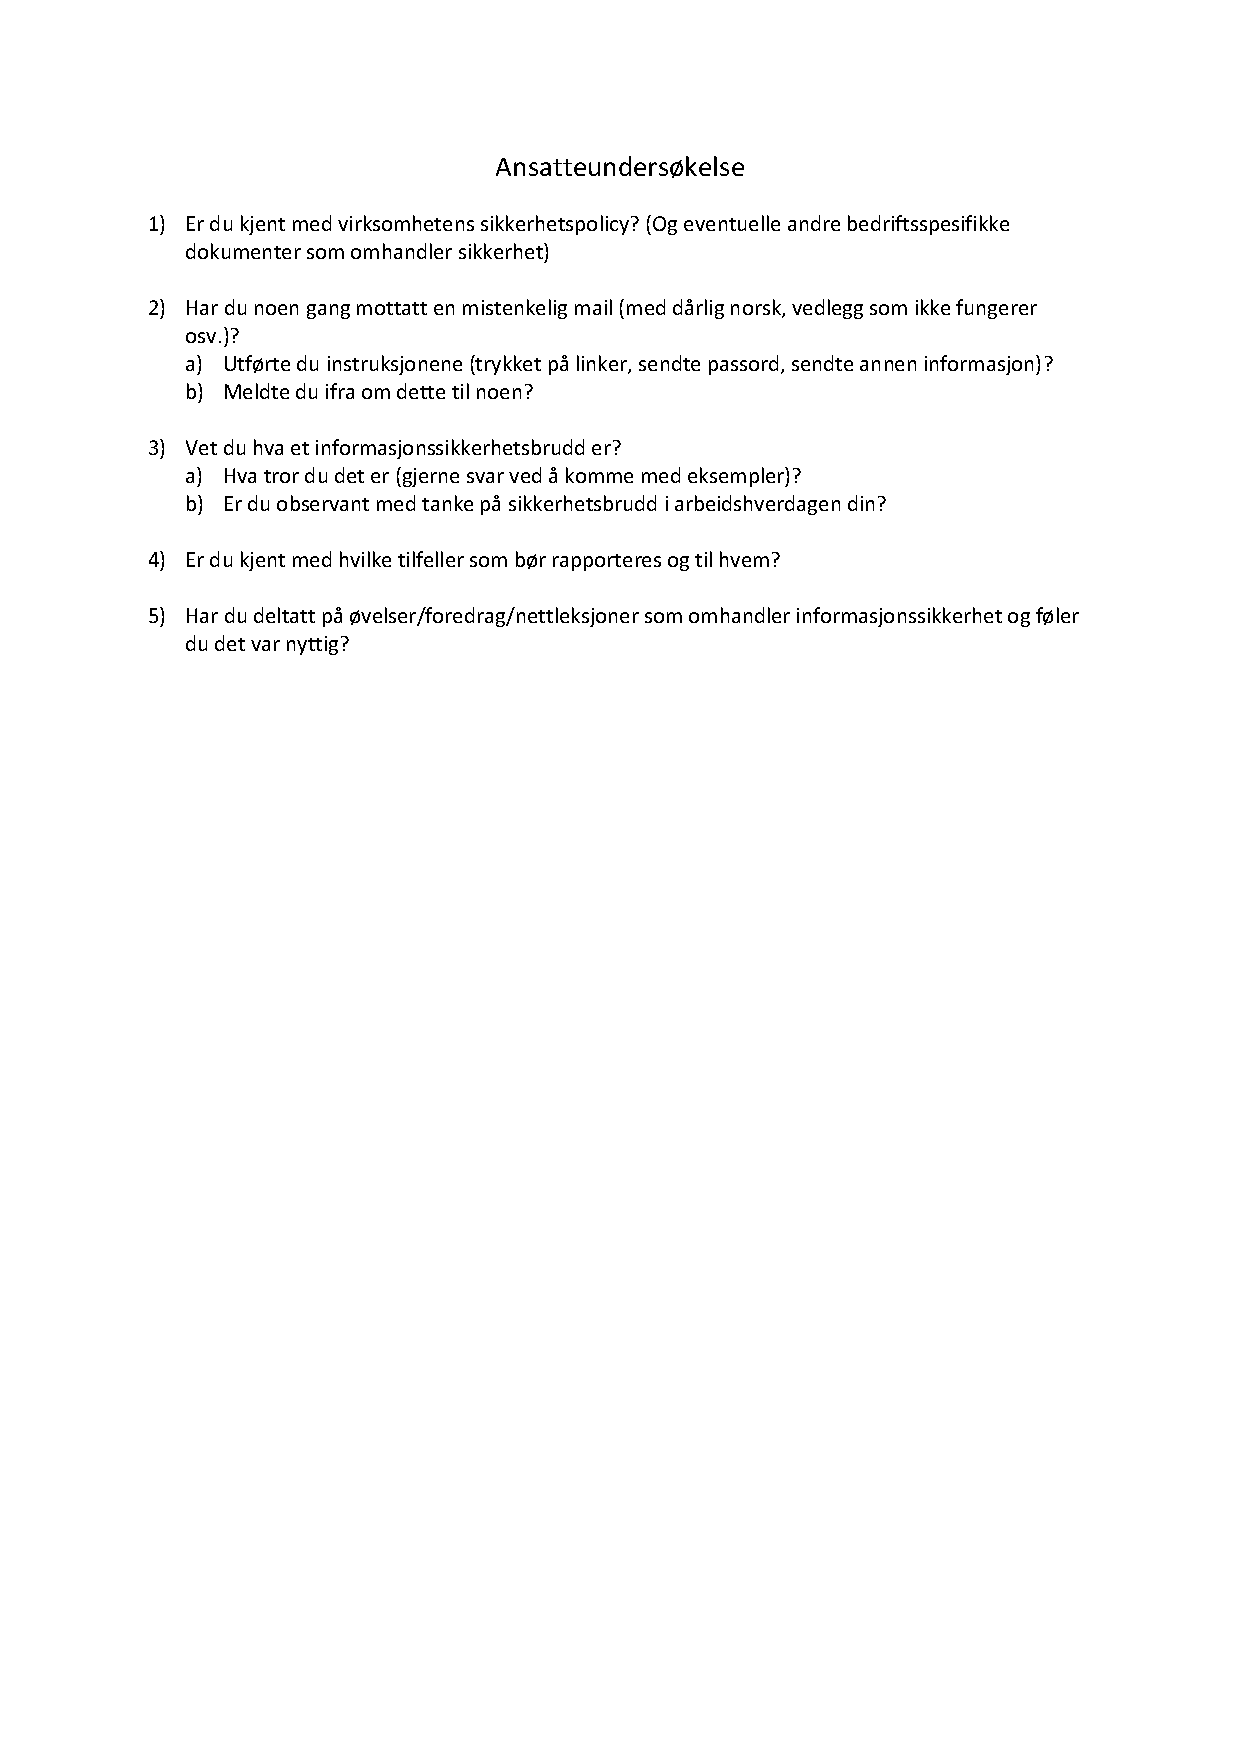
\includepdf[pages={-}]{Ansatteundersokelse.pdf}
\end{document}